% Arquivo LaTeX de exemplo de dissertação/tese a ser apresentados à CPG do IME-USP
% 
% Versão 5: Sex Mar  9 18:05:40 BRT 2012
%
% Criação: Jesús P. Mena-Chalco
% Revisão: Fabio Kon e Paulo Feofiloff
%  
% Obs: Leia previamente o texto do arquivo README.txt

\documentclass[11pt,twoside,a4paper]{book}

% ---------------------------------------------------------------------------- %
% Pacotes
\usepackage[T1]{fontenc}

%\usepackage[brazil,greek,english]{babel}
%\usepackage[brazil]{babel}
\usepackage[english]{babel}
%\usepackage[latin1]{inputenc}
\usepackage[utf8]{inputenc}
%\usepackage[LGRx, T1]{fontenc}
%\usepackage{textcomp}

%\usepackage[T1]{fontenc}
%\usepackage[brazil]{babel}
%\usepackage[latin1]{inputenc}

\usepackage[pdftex]{graphicx}           % usamos arquivos pdf/png como figuras
\usepackage{setspace}                   % espaçamento flexível
\usepackage{indentfirst}                % indentação do primeiro parágrafo
\usepackage{makeidx}                    % índice remissivo
\usepackage[nottoc]{tocbibind}          % acrescentamos a bibliografia/indice/conteudo no Table of Contents
\usepackage{courier}                    % usa o Adobe Courier no lugar de Computer Modern Typewriter
\usepackage{type1cm}                    % fontes realmente escaláveis
\usepackage{listings}                   % para formatar código-fonte (ex. em Java)
\usepackage{titletoc}
%\usepackage[bf,small,compact]{titlesec} % cabeçalhos dos títulos: menores e compactos
\usepackage[fixlanguage]{babelbib}
\usepackage[font=small,format=plain,labelfont=bf,up,textfont=it,up]{caption}
\usepackage[usenames,svgnames,dvipsnames]{xcolor}
\usepackage[a4paper,top=2.54cm,bottom=2.0cm,left=2.0cm,right=2.54cm]{geometry} % margens
%\usepackage[pdftex,plainpages=false,pdfpagelabels,pagebackref,colorlinks=true,citecolor=black,linkcolor=black,urlcolor=black,filecolor=black,bookmarksopen=true]{hyperref} % links em preto
\usepackage[pdftex,plainpages=false,pdfpagelabels,pagebackref,colorlinks=true,citecolor=DarkGreen,linkcolor=NavyBlue,urlcolor=DarkRed,filecolor=green,bookmarksopen=true]{hyperref} % links coloridos
\usepackage[all]{hypcap}                    % soluciona o problema com o hyperref e capitulos
\usepackage[round,sort,nonamebreak]{natbib} % citação bibliográfica textual(plainnat-ime.bst)
\bibpunct{(}{)}{;}{a}{\hspace{-0.7ex},}{,} % estilo de citação. Veja alguns exemplos em http://merkel.zoneo.net/Latex/natbib.php

\fontsize{60}{62}\usefont{OT1}{cmr}{m}{n}{\selectfont}

% ---------------------------------------------------------------------------- %
% Cabeçalhos similares ao TAOCP de Donald E. Knuth
\usepackage{fancyhdr}
\pagestyle{fancy}
\fancyhf{}
\renewcommand{\chaptermark}[1]{\markboth{\MakeUppercase{#1}}{}}
\renewcommand{\sectionmark}[1]{\markright{\MakeUppercase{#1}}{}}
\renewcommand{\headrulewidth}{0pt}

% ---------------------------------------------------------------------------- %
\graphicspath{{./images/}}             % caminho das figuras (recomendável)
\frenchspacing                          % arruma o espaço: id est (i.e.) e exempli gratia (e.g.) 
\urlstyle{same}                         % URL com o mesmo estilo do texto e não mono-spaced
\makeindex                              % para o índice remissivo
\raggedbottom                           % para não permitir espaços extra no texto
\fontsize{60}{62}\usefont{OT1}{cmr}{m}{n}{\selectfont}
\cleardoublepage
\normalsize

% ---------------------------------------------------------------------------- %
% Opções de listing usados para o código fonte
% Ref: http://en.wikibooks.org/wiki/LaTeX/Packages/Listings
\lstset{ %
	language=Java,                  % choose the language of the code
	basicstyle=\footnotesize,       % the size of the fonts that are used for the code
	numbers=left,                   % where to put the line-numbers
	numberstyle=\footnotesize,      % the size of the fonts that are used for the line-numbers
	stepnumber=1,                   % the step between two line-numbers. If it's 1 each line will be numbered
	numbersep=5pt,                  % how far the line-numbers are from the code
	showspaces=false,               % show spaces adding particular underscores
	showstringspaces=false,         % underline spaces within strings
	showtabs=false,                 % show tabs within strings adding particular underscores
	frame=single,	                % adds a frame around the code
	framerule=0.6pt,
	tabsize=2,	                    % sets default tabsize to 2 spaces
	captionpos=b,                   % sets the caption-position to bottom
	breaklines=true,                % sets automatic line breaking
	breakatwhitespace=false,        % sets if automatic breaks should only happen at whitespace
	escapeinside={\%*}{*)},         % if you want to add a comment within your code
	backgroundcolor=\color[rgb]{1.0,1.0,1.0}, % choose the background color.
	rulecolor=\color[rgb]{0.8,0.8,0.8},
	extendedchars=true,
	xleftmargin=10pt,
	xrightmargin=10pt,
	framexleftmargin=10pt,
	framexrightmargin=10pt
}






%%%%%%%%%%%%%%%%%% dj

\usepackage{nomencl}
\usepackage{tabu}
\usepackage{longtable}
\usepackage{ragged2e}
\usepackage{array}
\usepackage{multirow}
\usepackage{changepage}
\usepackage{pdfpages} % Para importar PDFs
\usepackage{booktabs} % Para tabela de sensores
\usepackage{siunitx} % Para tabela do N95
\usepackage{longtable} % Para tabelas ocuparem mais de uma página
\usepackage{usebib} % Para citar titulo de artigo no texto
\usepackage[]{epigraph}
\bibinput{thesisbib} 

\makenomenclature
\renewcommand{\nomname}{Nomenclatures}

\setlength{\headheight}{25pt}% corrige erro do fancyhdr

\newcommand{\paragraphdesc}[1]{
	% comentar a linha abaixo para ocultar descrição de parágrafos
%	\addcontentsline{toc}{subsection}{- #1} 
}

\usepackage{listings}
\lstloadlanguages{Ruby} % codigo usado em Touches On The Line
\usepackage{fancyvrb}

\usepackage{subcaption}


\usepackage{tablefootnote}


\usepackage{booktabs}  % nice looking tables
\usepackage{siunitx}
% \usepackage{fixltx2e}

\usepackage[section]{placeins}


%%%%%%%%%%%%%%%%%% dj-end





% ---------------------------------------------------------------------------- %
% Corpo do texto
\begin{document}
	\frontmatter 
	% cabeçalho para as páginas das seções anteriores ao capítulo 1 (frontmatter)
	\fancyhead[RO]{{\footnotesize\rightmark}\hspace{2em}\thepage}
	\setcounter{tocdepth}{2}
	\fancyhead[LE]{\thepage\hspace{2em}\footnotesize{\leftmark}}
	\fancyhead[RE,LO]{}
	\fancyhead[RO]{{\footnotesize\rightmark}\hspace{2em}\thepage}
	
	\onehalfspacing  % espaçamento
	
	% ---------------------------------------------------------------------------- %
	% CAPA
	% Nota: O título para as dissertações/teses do IME-USP devem caber em um 
	% orifício de 10,7cm de largura x 6,0cm de altura que há na capa fornecida pela SPG.
	% \thispagestyle{empty}
	% \begin{center}
	%     \vspace*{2.3cm}
	%     \textbf{\Large{Mobile Technologies for Music Interaction}}\\
	
	%     \vspace*{1.2cm}
	%     \Large{Antonio Deusany de Carvalho Junior}
	
	%     \vskip 2cm
	%     \textsc{
	%     Tese apresentada\\[-0.25cm] 
	%     ao\\[-0.25cm]
	%     Instituto de Matemática e Estatística\\[-0.25cm]
	%     da\\[-0.25cm]
	%     Universidade de São Paulo\\[-0.25cm]
	%     para\\[-0.25cm]
	%     obtenção do título\\[-0.25cm]
	%     de\\[-0.25cm]
	%     Doutor em Ciências}
	
	%     \vskip 1.5cm
	%     Programa: Pós-Graduação em Ciência da Computação\\
	%     Orientador: Prof. Dr. Marcelo Gomes de Queiroz
	
	%    	\vskip 1cm
	%     \normalsize{Durante o desenvolvimento deste trabalho o autor recebeu auxílio
	%     financeiro da CAPES}
	
	%     \vskip 0.5cm
	%     \normalsize{São Paulo, fevereiro de 2017}
	% \end{center}
	
	
	%--- English version ---%
	\thispagestyle{empty}
	\begin{center}
		\vspace*{2.3cm}
		\textbf{\Large{Mobile Technologies for Music Interaction}}\\
		
		\vspace*{1.2cm}
		\Large{Antonio Deusany de Carvalho Junior}
		
		\vskip 2cm
		%%MQZ: Esse modelo é oficial? Parece bizarro essa alternância entre português e inglês. Além disso tenho quase certeza que o título seria "Doctor of Science" e não "Science Doctor".
		\textsc{
			Thesis presented\\[-0.25cm] 
			to\\[-0.25cm]
			Instituto de Matemática e Estatística\\[-0.25cm]
			from\\[-0.25cm]
			Universidade de São Paulo\\[-0.25cm]
            in\\[-0.25cm]
            partial fulfillment\\[-0.25cm]
			for the\\[-0.25cm]
			requirements of the degree\\[-0.25cm]
			of\\[-0.25cm]
			Doctor of Science}
		
		\vskip 1.5cm
		Program: Pós-Graduação em Ciência da Computação\\
		Advisor: Prof. Dr. Marcelo Gomes de Queiroz
		
		\vskip 1cm
		\normalsize{During this work, the author received scholarship from CAPES}
		
		\vskip 0.5cm
		\normalsize{São Paulo, May 2017}
	\end{center}
	
	% ---------------------------------------------------------------------------- %
	% Página de rosto (SÓ PARA A VERSÃO DEPOSITADA - ANTES DA DEFESA)
	% Resolução CoPGr 5890 (20/12/2010)
	%
	% IMPORTANTE:
	%   Coloque um '%' em todas as linhas
	%   desta página antes de compilar a versão
	%   final, corrigida, do trabalho
	%
	%
	% \newpage
	% \thispagestyle{empty}
	%     \begin{center}
	%         \vspace*{2.3 cm}
	%         \textbf{\Large{Mobile Technologies for Music Interaction}}\\
	%         \vspace*{2 cm}
	%     \end{center}
	
	%     \vskip 2cm
	
	%     \begin{flushright}
	% 	Esta é a versão original da tese elaborada pelo\\
	% 	candidato Antonio Deusany de Carvalho Junior, tal como \\
	% 	submetida à Comissão Julgadora.
	%     \end{flushright}
	
	% \pagebreak
	%--- English version ---%
%	\newpage
%	\thispagestyle{empty}
%	\begin{center}
%		\vspace*{2.3 cm}
%		\textbf{\Large{Mobile Technologies for Music Interaction}}\\
%		\vspace*{2 cm}
%	\end{center}
%	
%	\vskip 2cm
%	
%	\begin{flushright}
%		This is the original version of the thesis written by\\
%		the candidate Antonio Deusany de Carvalho Junior\\
%		submitted to the Judging Committee. %%MQZ: reconfirmar (era Commission)
%	\end{flushright}
%	
%	\pagebreak
	
	
	% ---------------------------------------------------------------------------- %
	% Página de rosto (SÓ PARA A VERSÃO CORRIGIDA - APÓS DEFESA)
	% Resolução CoPGr 5890 (20/12/2010)
	%
	% Nota: O título para as dissertações/teses do IME-USP devem caber em um 
	% orifício de 10,7cm de largura x 6,0cm de altura que há na capa fornecida pela SPG.
	%
	% IMPORTANTE:
	%   Coloque um '%' em todas as linhas desta
	%   página antes de compilar a versão do trabalho que será entregue
	%   à Comissão Julgadora antes da defesa
	%
	%
	\newpage
	\thispagestyle{empty}
	    \begin{center}
	        \vspace*{2.3 cm}
	        \textbf{\Large{Mobile Technologies for Music Interaction}}\\
	        \vspace*{2 cm}
	    \end{center}
	
	    \vskip 2cm
	
	    \begin{flushright} 
	    This thesis version contains the changes, corrections, and suggestions\\%Esta versão da dissertação/tese contém as correções e alterações sugeridas\\
		from the Judging Commission during the defense of the original version\\%pela Comissão Julgadora durante a defesa da versão original do trabalho,\\
		that took place on May 24th, 2017. One copy of the original version is available at\\ %realizada em 14/12/2010. Uma cópia da versão original está disponível no\\
		the Instituto de Matemática e Estatística from Universidade de São Paulo.% Instituto de Matemática e Estatística da Universidade de São Paulo.
		
	
	    \vskip 2cm
	
	    \end{flushright}
	    \vskip 4.2cm
	
	    \begin{quote}
	    \noindent Judging Commission:
	    
	    \begin{itemize}
			\item Prof. Dr. Marcelo Gomes de Queiroz (advisor) - IME-USP
			\item Prof. Dr. Alfredo Goldman vel Lejbman - IME-USP
			\item Prof. Dr. Daniel Macêdo Batista - IME-USP
			\item Prof. Dr. Georg Essl - University of Wisconsin-Milwaukee
			\item Prof. Dr. Jason Freeman - Georgia Tech
	    \end{itemize}
	      
	    \end{quote}
	\pagebreak
	
	
	\pagenumbering{roman}     % começamos a numerar 
	
	% ---------------------------------------------------------------------------- %
	% Agradecimentos:
	% Se o candidato não quer fazer agradecimentos, deve simplesmente eliminar esta página 
	% \chapter*{Agradecimentos}
	% Texto texto texto texto texto texto texto texto texto texto texto texto texto
	% texto texto texto texto texto texto texto texto texto texto texto texto texto
	% texto texto texto texto texto texto texto texto texto texto texto texto texto
	% texto texto texto texto. Texto opcional.
	
	
	% ---------------------------------------------------------------------------- %
	
	% ---------------------------------------------------------------------------- %
	% Abstract
	\chapter*{Abstract}
	\noindent DE CARVALHO JUNIOR, A. D. \textbf{Mobile Technologies for Music Interaction}. 
	2017. 160 p.
	Thesis (Doctorate) - Instituto de Matemática e Estatística,
	Universidade de São Paulo, São Paulo, 2017.
	\\
	
	% Introduction
	Mobile music applications are becoming commonplace around the world, and mobile devices are used as digital instruments everywhere.
	Controlling, performing, or composing music in real time with these devices encourages collaboration and interaction, as telecommunication improvements allow many people to cooperate through local networks or the Internet.
	In this context, the aim of this thesis is to evaluate mobile technologies that might be suitable for mobile musicians and their audiences while performing or composing.
	% Objectives
	Specifically, the main goal is to explore technologies for collaborative mobile music and to obtain quantitative and qualitative data regarding these technologies and their settings, so that composers might take full advantage of the available options for mobile applications.
	% Methods
	This evaluation focuses on message exchange using Multicast, Unicast, and Cloud Services, using academic networks as the main pathway.
	With these services, messages are organized as packet streams, characterized by different sizes and time intervals.
	Evaluation also includes the development of several applications that make use of these technologies running on Android devices and web browsers. 
	These applications were used in actual performances, serving as both evaluation tools and experimental music instruments.
	% Results and Discussion
	The results were analyzed in terms of round trip time and data loss under very different configuration scenarios, demonstrating that although some obvious impediments cannot be circumvented (e.g. significant delays in international settings), it is possible to choose the specific technology and achieve interesting results under most music application scenarios.
	I argue that although in theory Multicast appears to be the best technology to use by far, it is the most difficult to implement due to the burden of configuring every step of the network pathway.
	On the other hand, Cloud Services are certainly slower than direct connections, but are the most compatible and easiest technology to set up, and are definitely suitable for many collaborative music experiences.
	% Conclusions
	To conclude, there is a discussion of how mobile music practitioners can take advantage of these results for composition and performance by considering specific technological advantages or drawbacks that are inherent to each technology and setting.
	\\
	
	\noindent \textbf{Keywords:} mobile music, computer music, computer networks, cloud services.
	
	% Resumo
	\chapter*{Resumo}
	
	\noindent DE CARVALHO JUNIOR, A. D. \textbf{Tecnologias Móveis para Interação Musical}. 
	2017. 160 f.
	Tese (Doutorado) - Instituto de Matemática e Estatística,
	Universidade de São Paulo, São Paulo, 2017.
	\\
	
	%Introduction
	Aplicações de Música Móvel estão se tornando populares ao redor do mundo e dispositivos móveis estão sendo utilizados como instrumentos musicais em diversos lugares.
	Controlar, apresentar ou compor música em tempo real com estes dispositivos estimula a colaboração e a interação, e os avanços nas telecomunicações permitem a um grande número de pessoas cooperar musicalmente através de redes locais ou da Internet.
	Neste contexto, o objetivo desta tese é avaliar as tecnologias móveis que podem ser úteis para músicos e público na performance ou na composição.
	% Objectives
	De maneira mais específica, o objetivo principal é explorar as tecnologias para Música Móvel colaborativa e obter resultados quantitativos e qualitativos referentes a estas tecnologias e suas configurações, de modo que compositores possam usufruir de todas as vantagens das opções para aplicações móveis.
	% Methods
	Esta avaliação enfoca a troca de mensagens através de Multicast, Unicast e Serviços em Nuvem utilizando redes de computadores acadêmicas como principal caminho.
	Através destes serviços as mensagens foram organizadas como fluxos de pacotes caracterizados por diversos tamanhos e intervalos entre envios.
	A avaliação também inclui o desenvolvimento de diversas aplicações fazendo uso destas tecnologias para dispositivos Android e navegadores Web, que foram utilizados em performances reais, servindo tanto como ferramentas de avaliação quanto como instrumentos para música experimental.
	% Results and Discussion
	Os dados são analisados com relação ao tempo de ida-e-volta e perda de pacotes em diferentes configurações de cenário, demonstrando que apesar de alguns impedimentos óbvios não poderem ser contornados (como o longo atraso em configurações internacionais, por exemplo), é possível escolher tecnologias adequadamente e alcançar resultados interessantes em muitos cenários de aplicações musicais.
	Argumento que apesar de em teoria o Multicast se apresentar de longe como a melhor tecnologia para estes cenários, ele é o mais difícil de ser implementado devido à grande complexidade na configuração de cada parte da rede para seu uso.
	Por outro lado, Serviços em Nuvem são certamente mais lentos, porém se apresentam como os mais compatíveis e fáceis de configurar, sendo definitivamente os mais adequados para muitas experiências de música colaborativa.
	% Conclusions
	Em conclusão, discuto como profissionais de Música Móvel podem se aproveitar dos resultados apresentados, considerando as vantagens e desvantagens tecnológicas específicas que são inerentes a cada tecnologia ou configuração quando utilizada em performances e composições musicais.
	\\
	
	\noindent \textbf{Palavras-chave:} música móvel, computação musical, redes de computadores, serviços de nuvens.
	
	% ---------------------------------------------------------------------------- %
	% Sumário
	\tableofcontents    % imprime o sumário
	
	% ---------------------------------------------------------------------------- %
	\chapter{List of Abbreviations}
	\begin{longtable}{ll}
		AC1750		& TP-Link AC1750 Archer C7 Wireless Dual Band Gigabit Router\\
        ADT         & Android Development Tools\\
		bps         & Bits per second\\
		CHI		    & ACM Conference on Human Factors in Computing Systems\\
		CIDR        & Classless Inter-Domain Routing\\
		Compmus		& Computer Music Research Group - IME --- USP\\
		D686		& LG D686 G Pro Lite Dual\\
		dBi         & Decibels Isotropic\\
		DSP		    & Digital Sound Processing\\
		ECA 	    & Escola de Comunicação e Artes --- USP\\	
		IrDA        & Infrared Data Association\\
		Gbps        & Gigabits per second\\
		I2		    & Internet2\\ 
		ICMC		& International Computer Music Conference\\
		IEEE        & Institute of Electrical and Electronics Engineers\\
		IEEE-SA     & IEEE Standards Association\\
		IME		    & Instituto de Matemática e Estatística --- USP\\
		ISM         & Industrial, scientific, and medical\\
		kbps        & Kilobits per second\\
		LAN         & Local Area Network\\
		MANET       & Mobile Ad-hoc Network\\
		MIS		    & \textit{Museu da Imagem e do Som de São Paulo} (São Paulo Museum of Image and Sound)\\ 
		MobileHCI	& ACM International Conference on Human-Computer Interaction with Mobile Devices and Services\\
		Mbps        & Megabits per second\\
		MIDI        & Musical Instrument Digital Interface\\
		MM          & Mobile Music\\
		MoPhO		& Mobile Phone Orchestra (Stanford University)\\
		MTU			& Maximum Transmission Unit\\
		MVC         & Model View Controller\\
		NFC         & Near Field Communication\\
		NIME		& Conference of New Interfaces for Music Expression\\
		NuSom		& Research Centre on Sonology - ECA --- USP\\
		OSC		    & Open Sound Control\\
		OTG         & USB On-The-Go\\
		P2P         & Peer to peer\\
		PDA		    & Personal digital assistant\\
		RAD		    & Rapid Application Development\\
		RNP		    & Rede Nacional de Ensino e Pesquisa (Brazilian National Research and Education Network)\\
		RoR		    & Ruby on Rails\\
		RTT		    & Round Trip Time\\
		S3		    & Samsung GT-I9300 Galaxy SIII\\
		SLA			& Service Layer Agreement\\
		SMC		    & Sound and Music Computing Conference\\
		ssh		    & Secure Shell\\
		UFPB	    & Universidade Federal da Paraíba\\
		UMich	    & University of Michigan\\
		USP         & Universidade de São Paulo\\
		VLAN        & Virtual LAN\\
		Z3		    & Sony D8533 (and D8503) Xperia Z3 Compact\\
		
		
		%          DFT         & Transformada discreta de Fourier (\emph{Discrete Fourier Transform})\\
	\end{longtable}
	\printnomenclature
	
	
	% ---------------------------------------------------------------------------- %
	% \chapter{Lista de Símbolos}
	% \begin{tabular}{ll}
	%         $\omega$    & Frequência angular\\
	%         $\psi$      & Função de análise \emph{wavelet}\\
	%         $\Psi$      & Transformada de Fourier de $\psi$\\
	% \end{tabular}
	
	% ---------------------------------------------------------------------------- %
	% Listas de figuras e tabelas criadas automaticamente
	\listoffigures            
	\listoftables            
	
	% ---------------------------------------------------------------------------- %
	% Capítulos do trabalho
	\mainmatter
	
	% cabeçalho para as páginas de todos os capítulos
	\fancyhead[RE,LO]{\thesection}
	
	\singlespacing              % espaçamento simples
	%\onehalfspacing            % espaçamento um e meio
% 	\doublespacing
	
	\input chapterIntro
	\input chapterMusic
 	\input chapterNetworks
    \input chapterResearch
% 	\input chapterApplications % moved to appendices
 	\input chapterEvaluations
 	%\input chapterResults
 	\input chapterConclusion
	
	% cabeçalho para os apêndices
	\renewcommand{\chaptermark}[1]{\markboth{\MakeUppercase{\appendixname\ \thechapter}} {\MakeUppercase{#1}} }
	\fancyhead[RE,LO]{}
	\appendix
	
	

\chapter{Evolution of smartphone features}
\label{ape:gsmarena-n95-s7}

Regarding the upgrades throughout the years we can see here that in 10 years the processors are almost 10 times faster in each core, the memory capacity is 25 times bigger now, and  the communication technologies increased the number of network bands and the bandwidth.
It is interesting to notice that in 2006 we already have a smartphone with WLAN, 3G, Bluetooth, infrared, GPS and radio technologies into a single board.

\begin{longtable}{llp{0.3\linewidth}p{0.3\linewidth}}
\caption{Communication technologies available on smartphones with 10 years announcement difference: Nokia N95 (2006) and Samsung Galaxy S7 (2016). Source: Adapted from \cite{GSMARENA2016-n95-s7}} \\ \hline
         &               & Nokia N95                                                   & Samsung Galaxy S7                                                                                                                                                                                                  \\ \hline \endhead
         
LAUNCH   & Announced     & 2006, September. Released 2007, March                        & 2016, February                                                                                                                                                                                              \\
         & Status        & Discontinued                                                 & Available. Released 2016, March                                                                                                                                                                             \\ \hline
         
PLATFORM & CPU           & 332 MHz Dual ARM 11                                          & Dual-core 2.15 GHz Kryo \& Dual-core 1.6 GHz Kryo or Quad-core 2.3 GHz Mongoose + Quad-core 1.6 GHz Cortex-A53                                                                                                                                                           \\ \hline
MEMORY   & Card slot     & microSD, up to 8 GB (dedicated slot), 128 MB included        & microSD, up to 200 GB (dedicated slot)                                                                                                                                                \\
         &               &                                                              & microSD, up to 200 GB                                                                                                                                                   \\
         & Internal      & 160 MB, 64 MB RAM                                            & 32/64 GB, 4 GB RAM                                                                                                                                                                                          \\ \hline
NETWORK  & Technology    & GSM / HSPA                                                   & GSM / HSPA / LTE                                                                                                                                                                                            \\
         & 2G bands      & GSM 850 / 900 / 1800 / 1900                                  & GSM 850 / 900 / 1800 / 1900                            \\
         & 3G Network    & HSDPA 2100                                                   & HSDPA 850 / 900 / 1700(AWS) / 1900 / 2100 - G930F                                                                                                                                                           \\
         &               & HSDPA 850 / 1900                          & TD-SCDMA                                                                                                                                                                                                    \\
         & 4G Network    &                                                              & LTE band 1(2100), 2(1900), 3(1800), 4(1700/2100), 5(850), 7(2600), 8(900), 12(700), 13(700), 17(700), 18(800), 19(800), 20(800), 25(1900), 26(850), 28(700), 38(2600), 39(1900), 40(2300), 41(2500) - G930F \\
         & Speed         & HSPA                                                         & HSPA 42.2/5.76 Mbps, LTE Cat9 450/50 Mbps                                                                                                                                                                   \\
         & GPRS          & Class 10                                                     & Yes                                                                                                                                                                                                         \\
         & EDGE          & Class 32, 296 kbps; DTM Class 11, 177 kbps                   & Yes                                                                                                                                                                                                         \\ \hline
COMMS    & WLAN          & Wi-Fi 802.11 b/g, UPnP technology                            & Wi-Fi 802.11 a/b/g/n/ac, dual-band, Wi-Fi Direct, hotspot                                                                                                                                                   \\
         & Bluetooth     & v2.0, A2DP                                                   & v4.2, A2DP, LE, aptX                                                                                                                                                                                        \\
         & GPS           & Yes, with A-GPS; Nokia Maps                                  & Yes, with A-GPS, GLONASS, BDS                                                                                                                                                                               \\
         & NFC           & No                                                           & Yes                                                                                                                                                                                                         \\
         & Infrared port & Yes                                                          & No                                                                                                                                                                                                          \\
         & Radio         & Stereo FM radio                                              & No                                                                                                                                                                                                          \\
         & USB           & miniUSB v2.0                                                 & microUSB v2.0, USB Host                                                                                                                                                                                     \\ \hline
\label{tab:gsmarena-n95-s7}
\end{longtable}





\chapter{Available sensors within the Android system}
\label{ape:android-sensors}

Here we have some sensors available for mobile devices, being the base sensors the ones that are related to physical sensors while the others are composite sensors that use values from the base sensors or merge two or more sensors.

% \begin{table}[]
% \centering

\begin{longtable}{@{}llllll@{}}
\caption{Definition of available sensors for Android system. Source: \cite{Android2016sensorssource,Android2016sensortypes}} \\ \hline
Sensor type                   & ID & \begin{tabular}[c]
{@{}l@{}}Reporting\\ mode\end{tabular} & \begin{tabular}[c]
{@{}l@{}}\# of \\ values\end{tabular} & \begin{tabular}[c]
{@{}l@{}}Composite\\ category\end{tabular} & \begin{tabular}[c]
{@{}l@{}}Low\\ power\end{tabular} \\ \hline \endhead
ACCELEROMETER                 & 1  & continuous   & 3         & (base sensor)    &           \\
GEOMAGNETIC\_FIELD            & 2  & continuous   & 3         & (base sensor)    &           \\
ORIENTATION                   & 3  & continuous   & 3         & attitude         &           \\
GYROSCOPE                     & 4  & continuous   & 3         & (base sensor)    &           \\
LIGHT                         & 5  & on-change    & 1         & (base sensor)    &           \\
PRESSURE                      & 6  & continuous   & 1         & (base sensor)    &           \\
TEMPERATURE                   & 7  &              & 1         &                  &           \\
PROXIMITY                     & 8  & on-change    & 1         & (base sensor)    &           \\
GRAVITY                       & 9  & continuous   & 3         & attitude         &           \\
LINEAR\_ACCELERATION          & 10 & continuous   & 3         & activity         &           \\
ROTATION\_VECTOR              & 11 & continuous   & 4         & attitude         &           \\
RELATIVE\_HUMIDITY            & 12 & on-change    & 1         & (base sensor)    &           \\
AMBIENT\_TEMPERATURE          & 13 & on-change    & 1         & (base sensor)    &           \\
MAGNETIC\_FIELD\_UNCALIBRATED & 14 & continuous   & 6         & uncalibrated     &           \\
GAME\_ROTATION\_VECTOR        & 15 & continuous   & 3         & attitude         &           \\
GYROSCOPE\_UNCALIBRATED       & 16 & continuous   & 6         & uncalibrated     &           \\
SIGNIFICANT\_MOTION           & 17 & one-shot     & 1         & activity         & yes       \\
STEP\_DETECTOR                & 18 & special      & 1         & activity         & yes       \\
STEP\_COUNTER                 & 19 & on-change    & 1         & activity         & yes       \\
GEOMAGNETIC\_ROTATION\_VECTOR & 20 & continuous   & 4         & attitude         & yes       \\
HEART\_RATE                   & 21 & on-change    & 1         & (base sensor)    &           \\
TILT\_DETECTOR                & 22 & special      & 1         & activity         & yes       \\
WAKE\_GESTURE                 & 23 & one-shot     & 1         & interaction      & yes       \\
GLANCE\_GESTURE               & 24 & one-shot     & 1         & interaction      & yes       \\
PICK\_UP\_GESTURE             & 25 & one-shot     & 1         & interaction      & yes       \\
WRIST\_TILT\_GESTURE          & 26 & special      & 1         &                  & yes       \\ \hline
\label{tab:android-sensors}
\end{longtable}




\chapter{Devices used during research}
\label{ape:gsmarena-lg-s3-z3}

The mobile devices used during this research were the LG D686 G Pro Dual Lite, Samsung GT-I9300 Galaxy SIII, and Sony Xperia D8533 (and D8503) Z3 Compact.
Their technical specifications are presented on the Table \ref{tab:gsmarena-lg-s3-z3}. 

\begin{longtable}{llp{0.2\linewidth}p{0.2\linewidth}p{0.2\linewidth}}
	\caption{Technical specifications of the mobile devices used during this research: D686, S3, and Z3. Source: Adapted from \cite{GSMARENA2017-lg-s3-z3}} \\ \hline
		&               & LG D686 G Pro Lite Dual                              & Samsung GT-I9300 Galaxy SIII                                                                  & Sony D8533 (and D8503) Xperia Z3 Compact                                                                                         \\ \hline \endhead
		NETWORK  & Technology    & GSM / HSPA                                      & GSM / HSPA                                                                                  & GSM / HSPA / LTE                                                                                               \\
		& 2G bands      & GSM 850 / 900 / 1800 / 1900 - SIM 1 \& SIM 2    & GSM 850 / 900 / 1800 / 1900                                                                 & GSM 850 / 900 / 1800 / 1900                                                                                    \\
		& 3G Network    & HSDPA 850 / 900 / 1900 / 2100                   & HSDPA 850 / 900 / 1900 / 2100                                                               & HSDPA 850 / 900 / 1700 / 1900 / 2100 - D5803                                                                   \\
		&               &                                                 &                                                                                             & HSDPA 850 / 900 / 1900 / 2100 - D5833                                                                          \\
		& 4G Network    &                                                 &                                                                                             & LTE band 1(2100), 2(1900), 3(1800), 4(1700/2100), 5(850), 7(2600), 8(900), 13(700), 17(700), 20(800) - D5803   \\
		&               &                                                 &                                                                                             & LTE band 1(2100), 3(1800), 5(850), 7(2600), 8(900), 28(700), 40(2300) - D5833                                  \\
		& Speed         & HSPA 7.2/5.76 Mbps                              & HSPA 21.1/5.76 Mbps                                                                         & HSPA 42.2/5.76 Mbps, LTE Cat4 150/50 Mbps                                                                      \\
		& GPRS          & Class 12                                        & Class 12                                                                                    & Up to 107 kbps                                                                                                 \\
		& EDGE          & Class 12                                        & Class 12                                                                                    & Up to 296 kbps                                                                                                 \\ \hline
		LAUNCH   & Announced     & 2013, October                                   & 2012, May                                                                                   & 2014, September                                                                                                \\
		& Status        & Available. Released 2013, November              & Available. Released 2012, May                                                               & Available. Released 2014, September                                                                            \\ \hline
		PLATFORM & OS            & Android OS, v4.1.2 (Jelly Bean)                 & Android OS, v4.0.4 (Ice Cream Sandwich), 4.3 (Jelly Bean)                                   & Android OS, v4.4.4 (KitKat), upgradable to v6.0 (Marshmallow)                                                  \\
		& Chipset       & Mediatek MT6577                                 & Exynos 4412 Quad                                                                            & Qualcomm MSM8974AC Snapdragon 801                                                                              \\
		& CPU           & Dual-core 1.0 GHz Cortex-A9                     & Quad-core 1.4 GHz Cortex-A9                                                                 & Quad-core 2.5 GHz Krait 400                                                                                    \\
		& GPU           & PowerVR SGX531                                  & Mali-400MP4                                                                                 & Adreno 330                                                                                                     \\ \hline
		MEMORY   & Card slot     & microSD, up to 32 GB (dedicated slot)           & microSD, up to 64 GB (dedicated slot)                                                       & microSD, up to 256 GB (dedicated slot)                                                                         \\
		& Internal      & 8 GB, 1 GB RAM                                  & 16/32/64 GB, 1 GB RAM                                                                       & 16 GB, 2 GB RAM                                                                                                \\ \hline
		COMMS    & WLAN          & Wi-Fi 802.11 b/g/n, Wi-Fi Direct, DLNA, hotspot & Wi-Fi 802.11 a/b/g/n, dual-band, Wi-Fi Direct, DLNA, hotspot                                & Wi-Fi 802.11 a/b/g/n/ac, dual-band, Wi-Fi Direct, DLNA, hotspot                                                \\
		& Bluetooth     & v3.0, A2DP                                      & v4.0, A2DP, EDR, aptX                                                                       & v4.0, A2DP, LE, aptX                                                                                           \\
		& GPS           & Yes, with A-GPS                                 & Yes, with A-GPS, GLONASS                                                                    & Yes, with A-GPS, GLONASS                                                                                       \\
		& NFC           &                                                 & Yes                                                                                         & Yes                                                                                                            \\
		& Infrared port & Yes                                             & No                                                                                          & No                                                                                                             \\
		& Radio         & FM radio                                        & Stereo FM radio, RDS                                                                        & Stereo FM radio, RDS                                                                                           \\
		& USB           & microUSB v2.0                                   & microUSB v2.0 (MHL TV-out), USB Host                                                        & microUSB v2.0 (MHL TV-out), USB Host; magnetic connector                                                       \\ \hline
		FEATURES & Sensors       & Accelerometer, proximity, compass               & Accelerometer, gyro, proximity, compass, barometer                                          & Accelerometer, gyro, proximity, compass, barometer                                                             \\ \hline
		BATTERY  &               & Removable Li-Ion 3140 mAh battery               & Removable Li-Ion 2100 mAh battery                                                           & Non-removable Li-Ion 2600 mAh battery                                                                          \\
		& Stand-by      & Up to 845 h                                     & Up to 590 h (2G) / Up to 790 h (3G)                                                         & Up to 880 h (2G) / Up to 920 h (3G)                                                                            \\
		& Talk time     & Up to 14 h 30 min                               & Up to 21 h 40 min (2G) / Up to 11 h 40 min (3G)                                             & Up to 12 h (2G) / Up to 14 h (3G)                                                                              \\
		& Music play    &                                                 &                                                                                             & Up to 110 h           \\ \hline                                                                                                                                                                                    
\label{tab:gsmarena-lg-s3-z3}
\end{longtable}



Two specific routers were bought in order to be used during the evaluation. 
One router was maintained at USP while the other was situated at UMich.
The technical details about the routers are described at Table \ref{tab:tplink-ac1750}.

\begin{longtable}{lp{0.7\linewidth}}		
\caption{Technical specifications of the TP-Link AC1750 Archer C7 Wireless Dual Band Gigabit Router. Source: Addapted from \cite{TPLINK2017AC1750}} \\ \hline
		HARDWARE FEATURES 		 		 		 		 & \\ 
		Interface 		 		 		 		 & 4 10/100/1000Mbps LAN Ports\\
													 & 1 10/100/1000Mbps WAN Port\\
													 & 2 USB 2.0 Ports \\
		Button 		 		 		 		 & WPS/Reset Button\\
												 & Wireless On/Off Switch \\
												 & Power On/Off Button \\
		External Power Supply 		 		 		 		 & 12VDC / 2A \\
		Dimensions ( W x D x H ) 		 		 		 		 & 9.6x6.4x1.3 in. (243x160.6x32.5mm) \\
		Antenna Type 		 		 		 		 & Three detachable antennas ( RP-SMA) \\ \hline
		WIRELESS FEATURES 		 		 		 		 & \\
		Wireless Standards 		 		 		 		 & IEEE 802.11ac/n/a 5GHz\\
																	 & IEEE 802.11b/g/n 2.4GHz \\
		Frequency 		 		 		 		 & 2.4GHz and 5GHz \\
		Signal Rate 		 		 		 		 		 & 5GHz: Up to 1300Mbps \\ 
		                                                    & 2.4GHz:  Up to 450Mbps \\
%		Reception Sensitivity 		 		 		 		 		 & 5GHz:\\ 
%																				& 11a 6Mbps: -96dBm\\ 
%																				& 11a 54Mbps: -79dBm \\ 
%																				& 11ac HT20: -71dBm \\
%																				& 11ac HT40: -66dBm \\
%																				& 11ac HT80: -63dBm\\
%																				& 2.4GHz: \\
%																				& 11g 54M: -77dBm\\
%																				& 11n HT20: -74dBm \\
%																				& 11n HT40: -72dBm \\
		Transmit Power 		 		 		 		 		 & CE: \\
																		& \textless20dBm(2.4GHz)\\
																		& \textless23dBm(5GHz) \\
																		& FCC:\\
																		& \textless30dBm \\
		Wireless Functions 		 		 		 		 		 & Enable/Disable Wireless Radio, WDS Bridge, WMM, Wireless Statistics \\
		Wireless Security 		 		 		 		 		 & 64/128-bit WEP, WPA / WPA2, WPA-PSK/ WPA2-PSK encryption \\ \hline
		SOFTWARE FEATURES 		 		 		 		 		 & \\
		Quality of Service 		 		 		 		 		 & WMM, Bandwidth Control \\
		WAN Type 		 		 		 		 		 & Dynamic IP/Static IP/PPPoE/PPTP(Dual Access)/L2TP(Dual Access)/BigPond \\
		Management 		 		 		 		 		 & Access Control\\
																	& Local Management\\
																	& Remote Management \\
		DHCP 		 		 		 		 		 & Server, Client, DHCP Client List, Address Reservation \\
		Port Forwarding 		 		 		 		 		 & Virtual Server, Port Triggering, UPnP, DMZ \\
		Dynamic DNS 		 		 		 		 		 & DynDns, Comexe, NO-IP \\
		VPN Pass-Through 		 		 		 		 		 & PPTP, L2TP, IPSec \\
		Access Control 		 		 		 		 		 & Parental Control, Local Management Control, Host List, Access Schedule, Rule Management \\
		Firewall Security 		 		 		 		 		 & DoS, SPI Firewall\\
																		& IP Address Filter/MAC Address Filter/Domain Filter\\
																		& IP and MAC Address Binding \\
		Protocols 		 		 		 		 		 & Supports IPv4 and IPv6 \\
		USB Sharing 		 		 		 		 		 & Support Samba(Storage)/FTP Server/Media Server/Printer Server \\
		Guest Network 		 		 		 		 		 & 2.4GHz guest network x 1 \\
																		& 5GHz guest network x 1 \\ \hline
		OTHERS 		 		 		 		 		 & \\
		Certification 		 		 		 		 		 & CE, FCC, RoHS \\ \hline
		\label{tab:tplink-ac1750}
\end{longtable}

%% ------------------------------------------------------------------------- %%
% \chapter{Emails contacted during the research}
% \label{ape:peoplecontacted}

% \begin{longtable}{lp{0.3\linewidth}p{0.3\linewidth}}
% 	\caption{People and emails contacted during research} \\ \hline
% 	Name & Information & Email    \\ \hline \endhead
% Alfredo Goldman vel Lejbman & Director of the Centro de Competência em Software Livre~(CCSL) at IME-USP & gold@ime.usp.br \\
% Multicast support at RNP & Email defined for asking for information regarding Multicast at RNP site & multicast-info@rnp.br  \\
% Multicast list at RNP & Discussion list about Multicast at RNP & majordomo@rnp.br\\
% Information email at RNP & Email available for asking for informations at RNP & info@rnp.br\\
% Helpdesk at RNP & Email used for the helpdesk at RNP & helpdesk@rt.rnp.br\\
% Lisandro Zambenedetti Granville & Co-Chair of the Network Management Research Group of the Internet Research Task Force & granville@inf.ufrgs.br\\
% José Luiz Ribeiro Filho & Director of Services and Solutions Board at RNP & jose.luiz@rnp.br\\
% Antônio Carlos Fernandes Nunes & Adjunct Director of Solutions Management Adjunct Board at RNP & antonio.nunes@rnp.br \\
% NOC - RNP & Network Operations Center contact at RNP & noc@rnp.br\\
% Fábio Rodrigues Ribeiro & Operations Analist at Operations Management of Network Engineering Management at RNP & fabio.ribeiro@rnp.br\\
% Edson Lima Monteiro (aka Boni) & Manager of the Backbone of USP and member of Seção Técnica de Configuração - Divisão de Comunicações - CCE - USP & boni@usp.br\\
% Luiz Eduardo Silva dos Santos & Departamento de Tecnologia da Informação - DTI - USP & lesantos@usp.br\\

% Henrique Cabral de Souza Rodrigues & Técnico em Informática - SI - IME - USP &hcabral@ime.usp.br \\
% & & admin@ime.usp.br\\
% Valter Pereira & & valter.pereira@pop-sp.rnp.br\\
% Wagner Pereira & & wagner.pereira@pop-sp.rnp.br\\
% Rogerio Herrera Mendonça & & rogerio.herrera@pop-sp.rnp.br\\
% Rogerio Herrera & & rogerio@pop-sp.rnp.br\\
% Andre Lopes da Silva & & alopes@ime.usp.br\\
% & & operacao@pop-sp.rnp.br\\
% Roy Hockett & Network Architect, ITS Communications Systems and Data Centers - University of Michigan & royboy@umich.edu\\
% ITSCommna & & itscommna@umich.edu\\

% & & decastro@usp.br\\
% Michael Stanton - RNP && michael@rnp.br\\
% & & noc@redclara.net\\
% & & noc@rnp.br\\
% & & neg@redclara.net\\
% & & rt@eecs.umich.ed\\
% Marco Antonio M. Teixeira & Diretoria Adjunta de Engenharia de Redes e Operações RNP – Rede Nacional de Ensino e Pesquisa & marco.teixeira@rnp.br\\

% William Alexandre Miura Gnann & & gnann@ime.usp.br\\
% Alex Moura & & alex.moura@rnp.br\\
 
% & & pop@pop-sp.rnp.br \\
% & & aluizio.hazin@rnp.br\\
 
% Brian Pullin & & bpullin@grnoc.iu.edu\\
% Brady Farver & & bfarver@umich.edu\\

% Guilherme Ladvocat & GO - Gerência de Operações - DAERO - Diretoria Adjunta de Engenharia de Redes e Operações - RNP - Rede Nacional de Ensino e Pesquisa &  guilherme.ladvocat@rnp.br\\

% Nathan Miller & Indiana University GlobalNOC - Internet2 Network Engineer & ndm2@globalnoc.iu.edu\\
% Christian O'Flaherty & Regional Development - Internet Society  & oflaherty@isoc.org\\
% Iara Machado & & iara@rnp.br\\
% Alex Soares de Moura & & alex@rnp.br\\

% Guillermo Cicileo & & guillermo@lacnic.net\\

%  Eric Boyd & &  eboyd@internet2.edu\\
 
% 		\label{tab:emailscontacted}
% \end{longtable}

% ------------------------------------------------------------------------- %%
 \chapter{Applications created during the research}
 \label{ape:applications}

\input chapterApplications


\chapter{Conference papers published about this research project}
\label{ape:papers}


%% ------------------------------------------------------------------------- %%
\section{SBCM 2013 - FFT benchmark on Android devices: Java versus JNI}
\label{ape:papersbcm2013}

\subsection*{Paper details}

Title: \textit{FFT benchmark on Android devices: Java versus JNI}

Authors: Antonio Deusany de Carvalho Junior, Max Rosan, André Bianchi, Marcelo Queiroz

\subsection*{Conference details}

Title: 14o Simpósio Brasileiro de Computação Musical~(SBCM)

Venue: Escola de Música de Brasília~(EMB), Brasília, DF, Brazil

Dates: October 31 to November 2, 2013

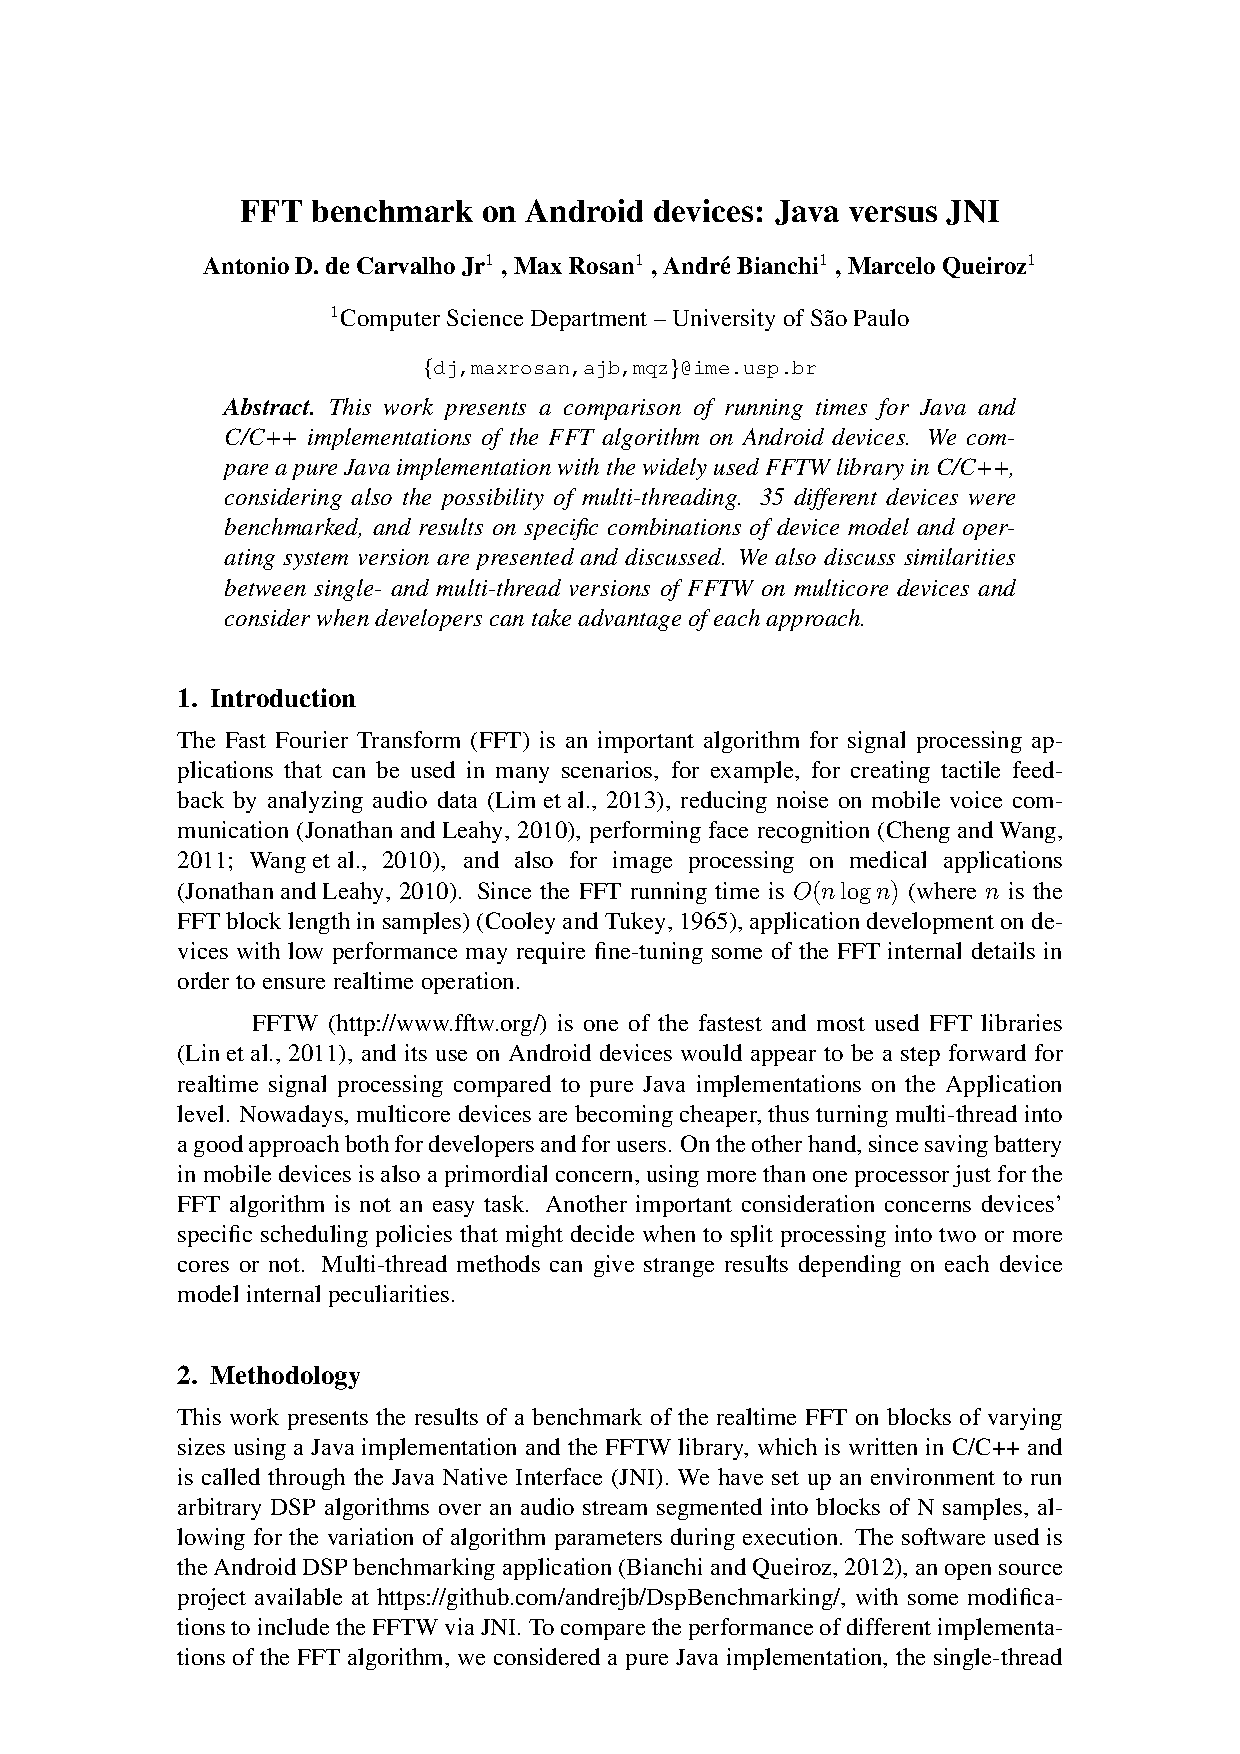
\includepdf[pages=-,frame,scale=0.8,pagecommand={}]{papers/2013-sbcm.pdf}

%% ------------------------------------------------------------------------- %%
\section{ICSC 2013 - Touches on the line: Sharing Csound scores using web server and mobile phones}
\label{ape:papericsc2013}

\subsection*{Paper details}

Title: \textit{Touches on the line: Sharing Csound scores using web server and mobile phones}

Authors: Antonio Deusany de Carvalho Junior

\subsection*{Conference details}

Title: 2nd International CSound Conference~(ICSC)

Venue: Berklee College of Music, Boston, MA, USA

Dates: October 25 to 27, 2013

\subsection*{Remarks}

During the conference, I performed at the Concert \#6 on October 27th with the application running on two mobile devices at the David Friend Recital Hall, Berklee College of Music, Boston, MA, USA~\footnote{\url{http://www.csounds.com/csound-conference-poster-schedule/}}.
This performance happened just before the concert in which performed Jean-Claude Risset, John Chowning, and Richard Boulanger, the masters of Computer Music that I met during this conference.

I also met two important woman for Computer Music during this conference.
Sitting by her side during concerts, I had a brief talk with Marjorie Matthews, the spouse of Max Matthews, the father of Computer Music.
The other woman was Judy Klein, a pianist and professor of electronic music.
We went out for a cup of tea and she exposed me the great history of Computer Music during the 1980's when she was working with the first versions of CSound and waiting the whole night to listen minutes of synthesized sounds.

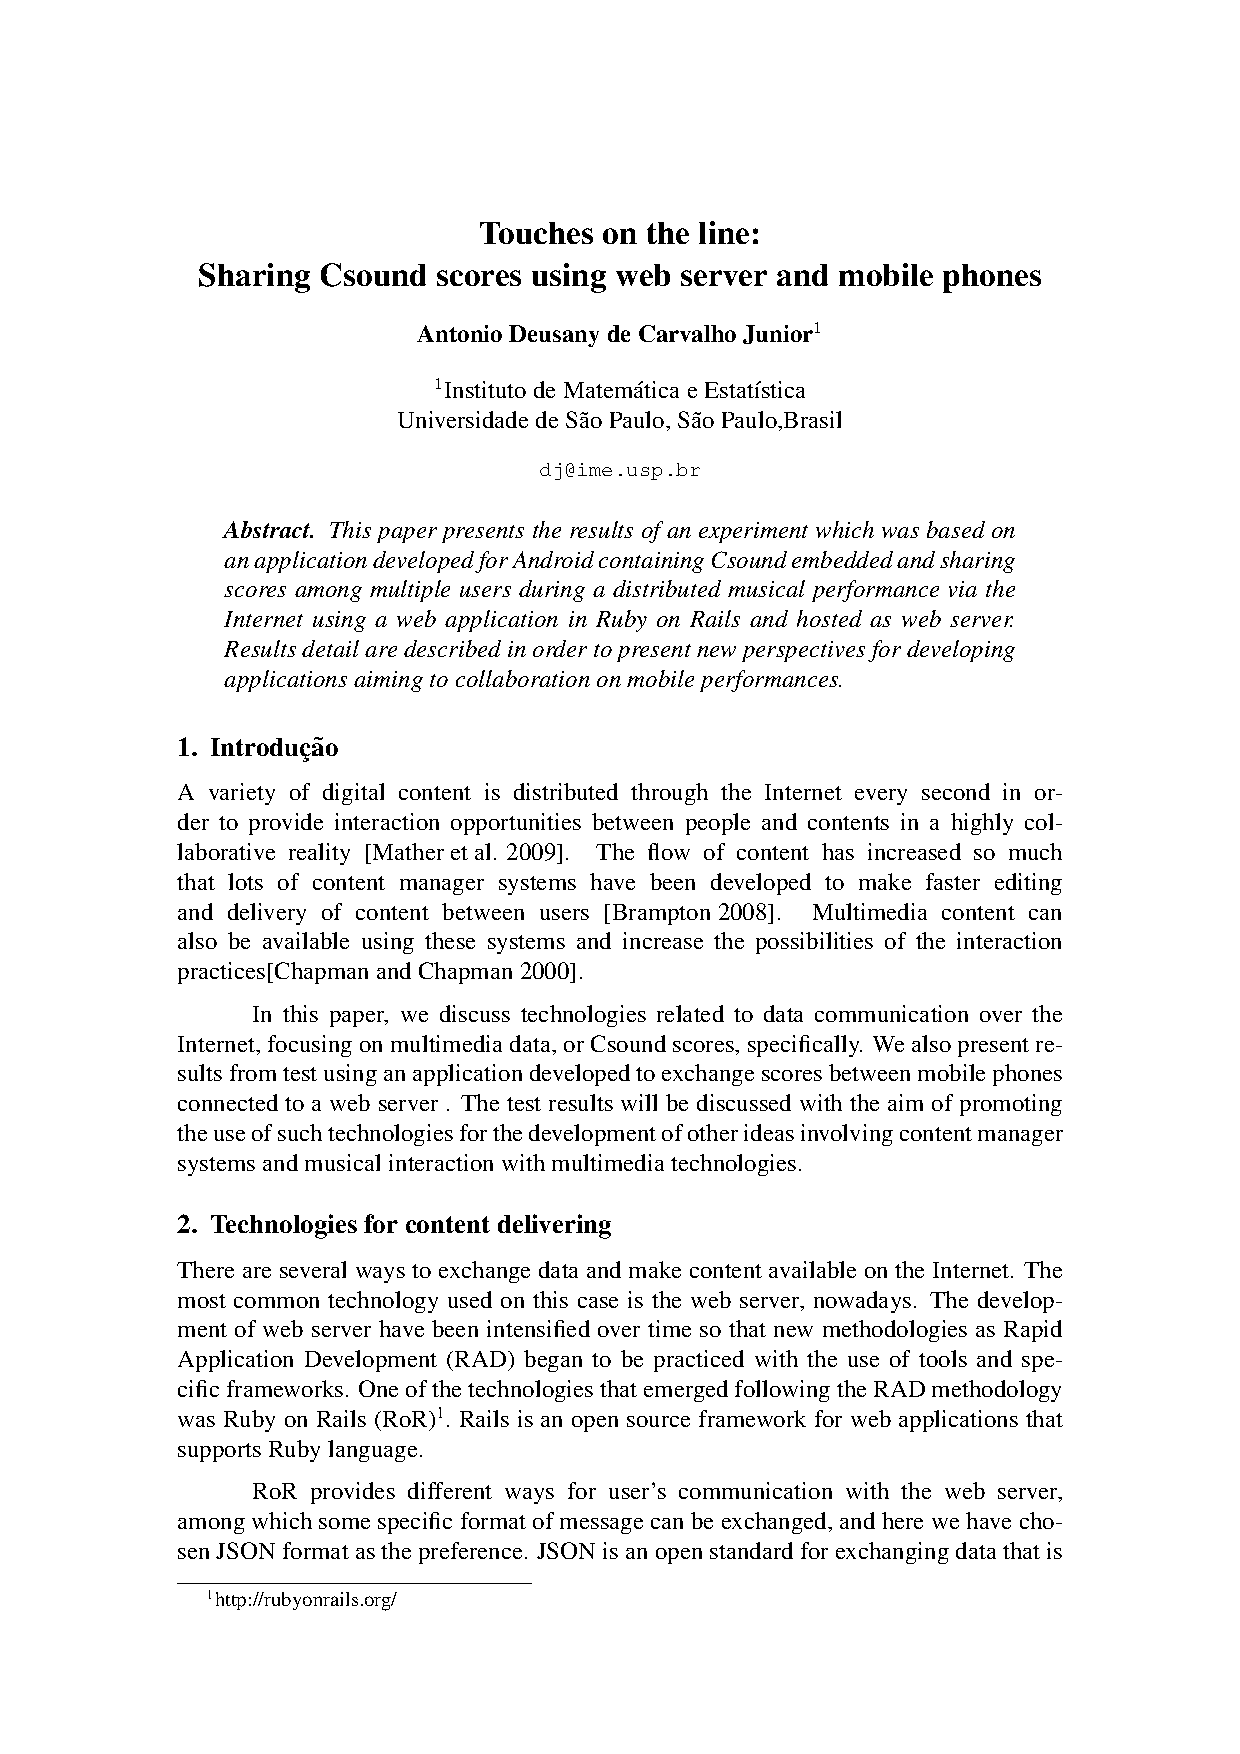
\includepdf[pages=-,frame,scale=0.8,pagecommand={}]{papers/2013-csound.pdf}

%% ------------------------------------------------------------------------- %%
\section{BATS 2014 - Notes on the Elimination of the Mobile Music Audience}
\label{ape:paperbats2014}

\subsection*{Paper details}

Title: \textit{Notes on the Elimination of the Mobile Music Audience}

Authors: André Damião Bandeira, Antonio Deusany de Carvalho Junior

\subsection*{Conference details}

Title: 14th Biennial Arts and Technology Symposium

Venue: Connecticut College, Ammerman Center for Arts and Technology, New London, CT

Dates: February 27, 28 and March 1, 2014


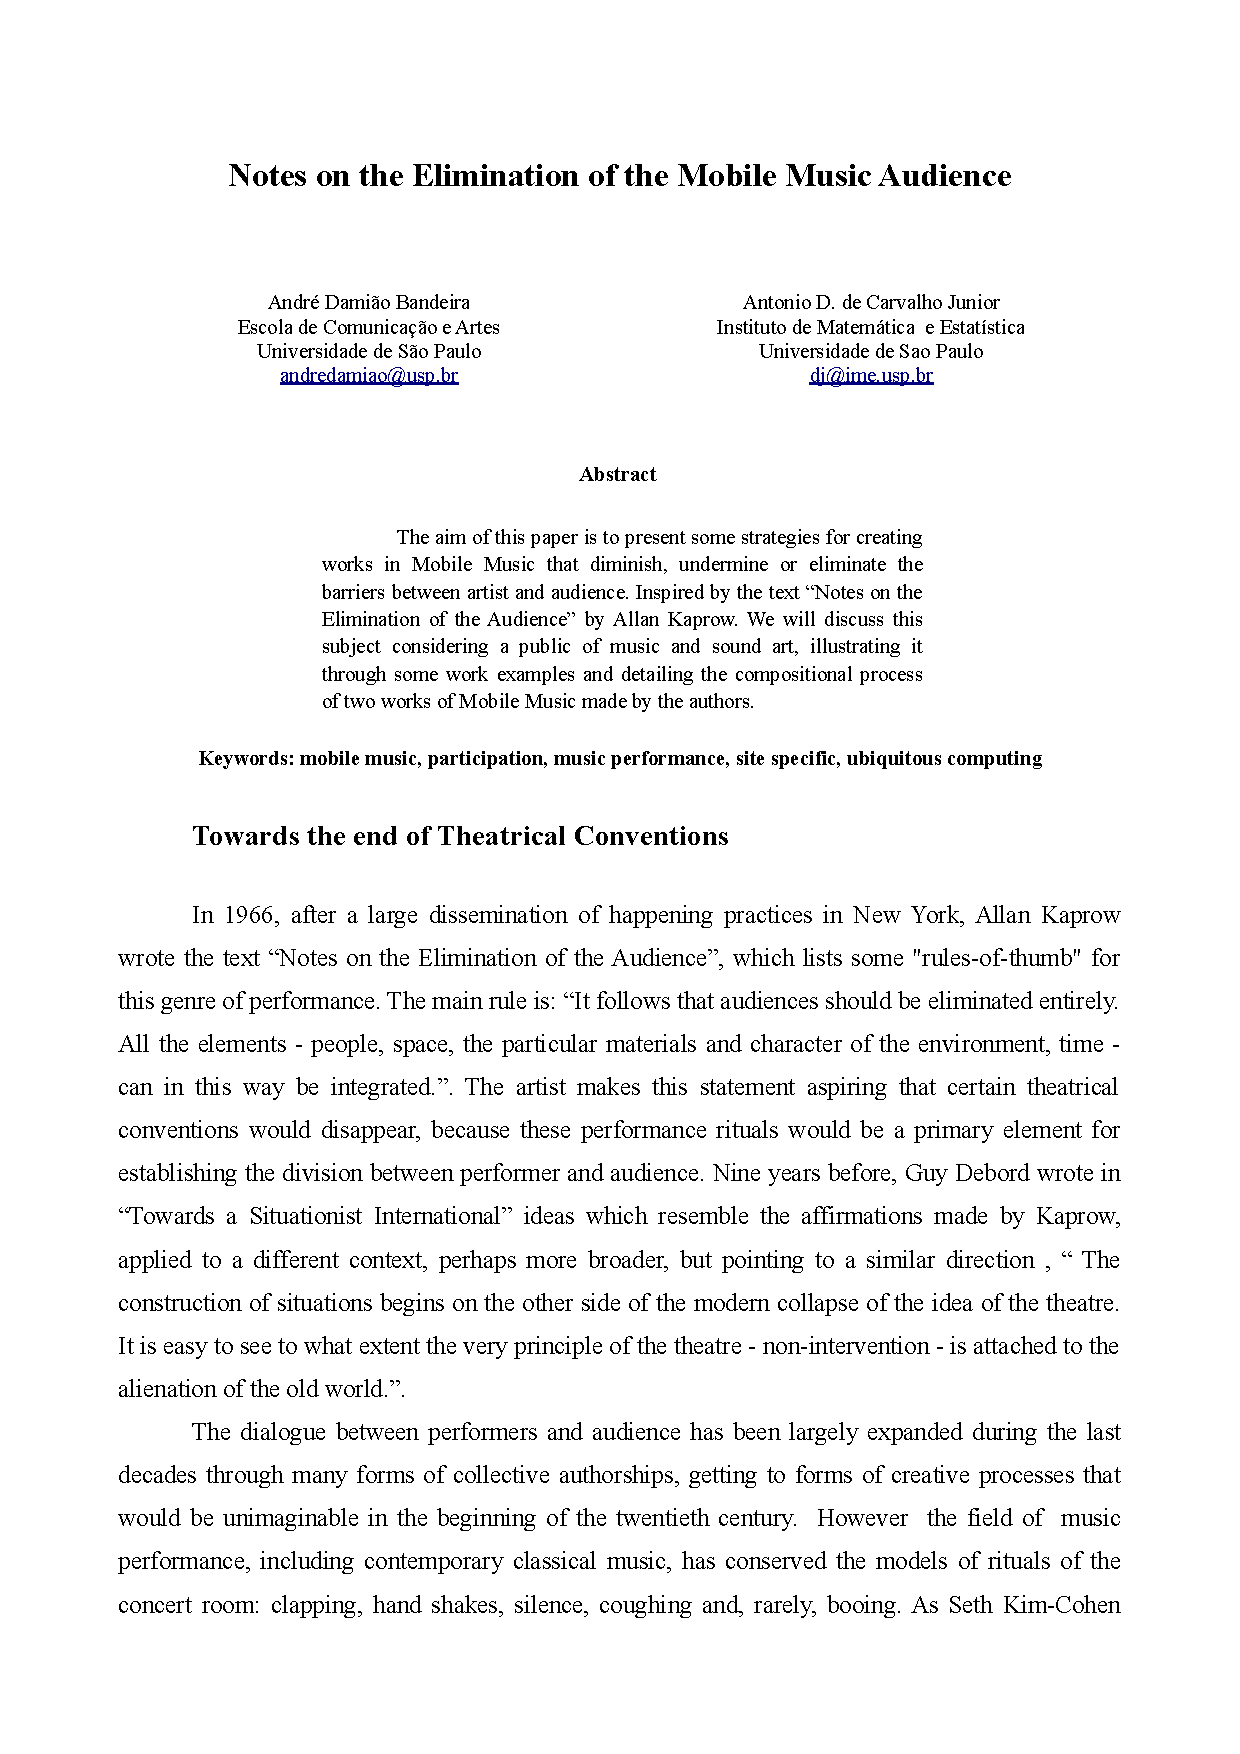
\includepdf[pages=-,frame,scale=0.8,pagecommand={}]{papers/2014-bienial-compressed.pdf}


%% ------------------------------------------------------------------------- %%
\section{ICMC 2014 - Sensors2PD: Mobile sensors and WiFi information as input for Pure Data}
\label{ape:papericmc2014}

\subsection*{Paper details}

Title: \textit{Sensors2PD: Mobile sensors and WiFi information as input for Pure Data}

Authors: Antonio Deusany de Carvalho Junior

\subsection*{Conference details}

Title: 40th International Computer Music Conference and 11th Sound and Music Computing Conference

Venue: Athens, Greece

Dates: September 14 to 20, 2014 

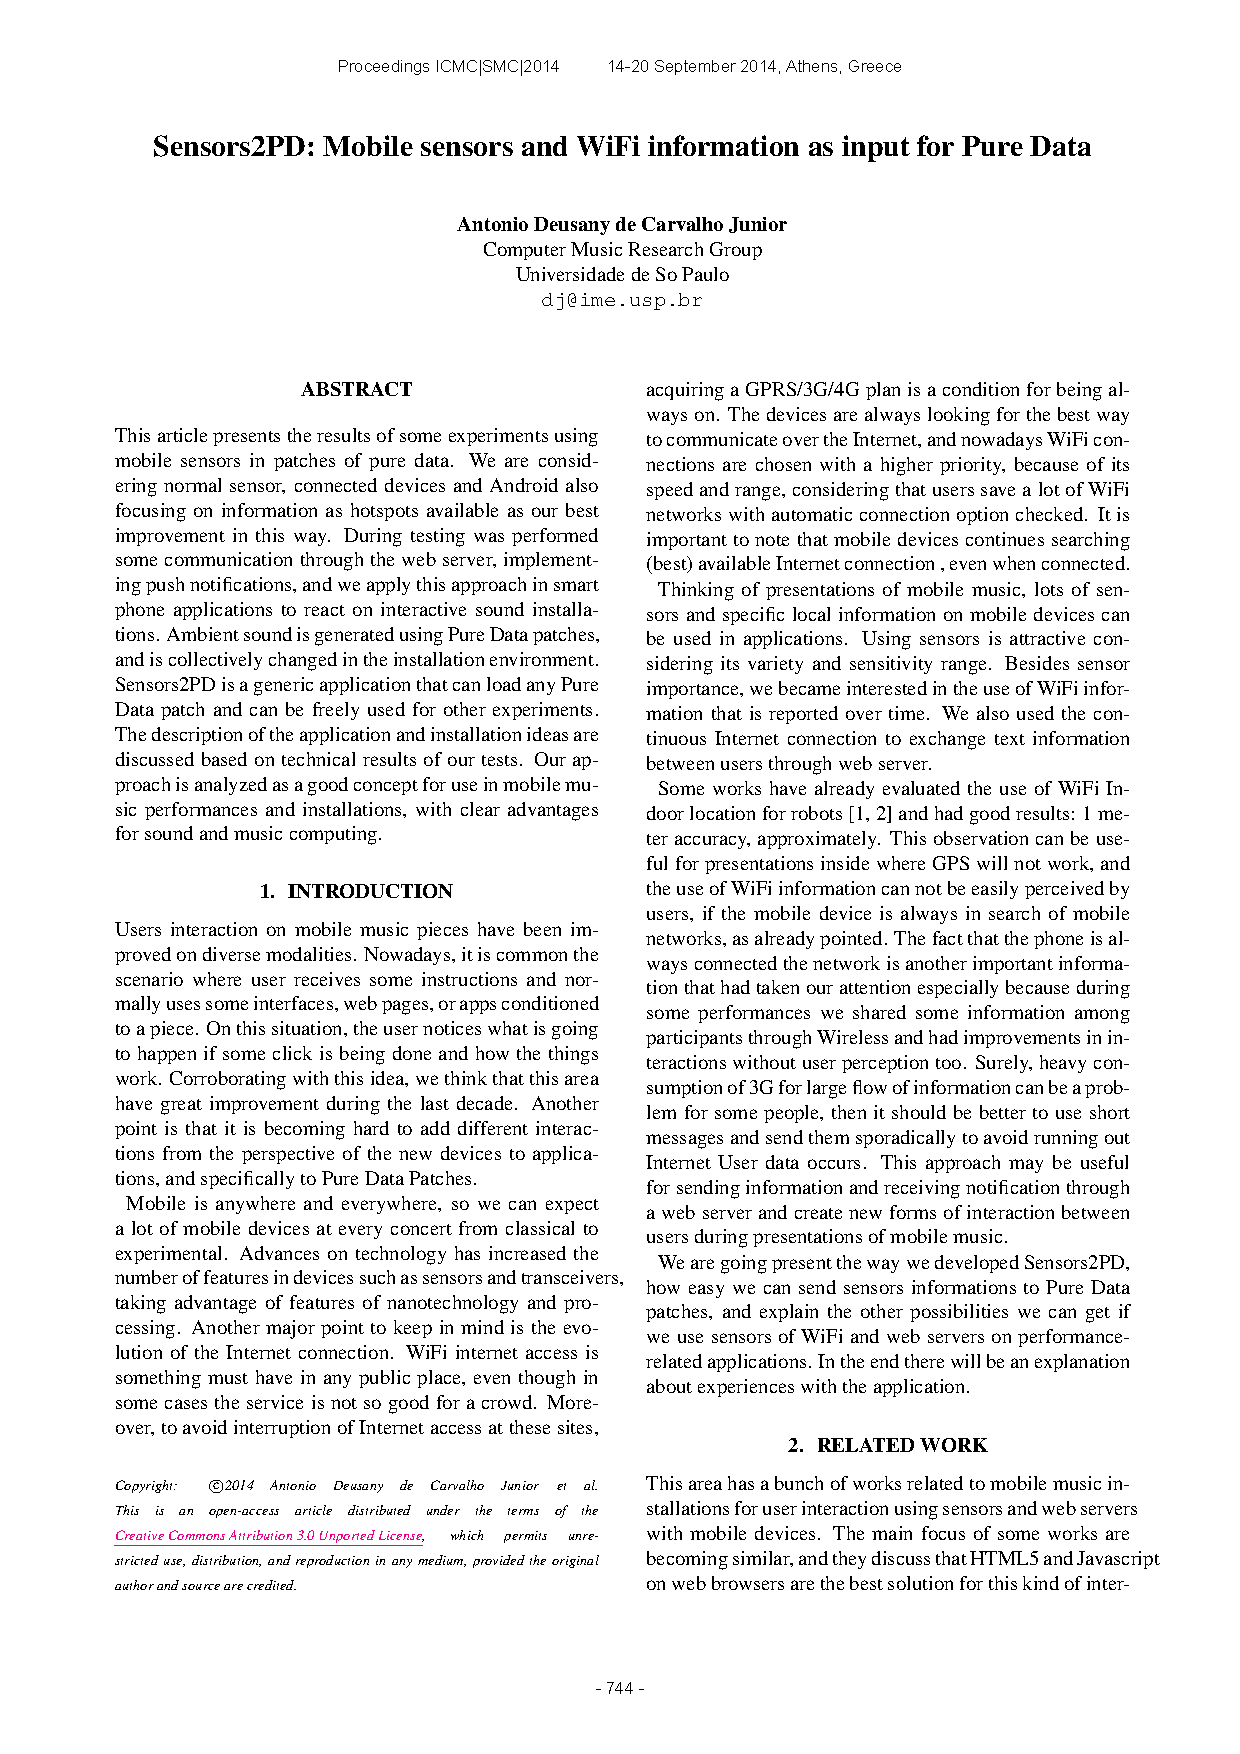
\includepdf[pages=-,frame,scale=0.8,pagecommand={}]{papers/2014-icmcsmc.pdf}

%% ------------------------------------------------------------------------- %%
\section{NIME 2015 - Indoor localization during installations using Wi-Fi}
\label{ape:papernime2015}

\subsection*{Paper details}

Title: \textit{Indoor localization during installations using Wi-Fi}

Authors: Antonio Deusany de Carvalho Junior

\subsection*{Conference details}

Title: 15th International Conference on New Interfaces for Musical Expression

Venue: Lousiana State University, Banton Rouge, LA, USA

Dates: May 31 to June 3, 2015

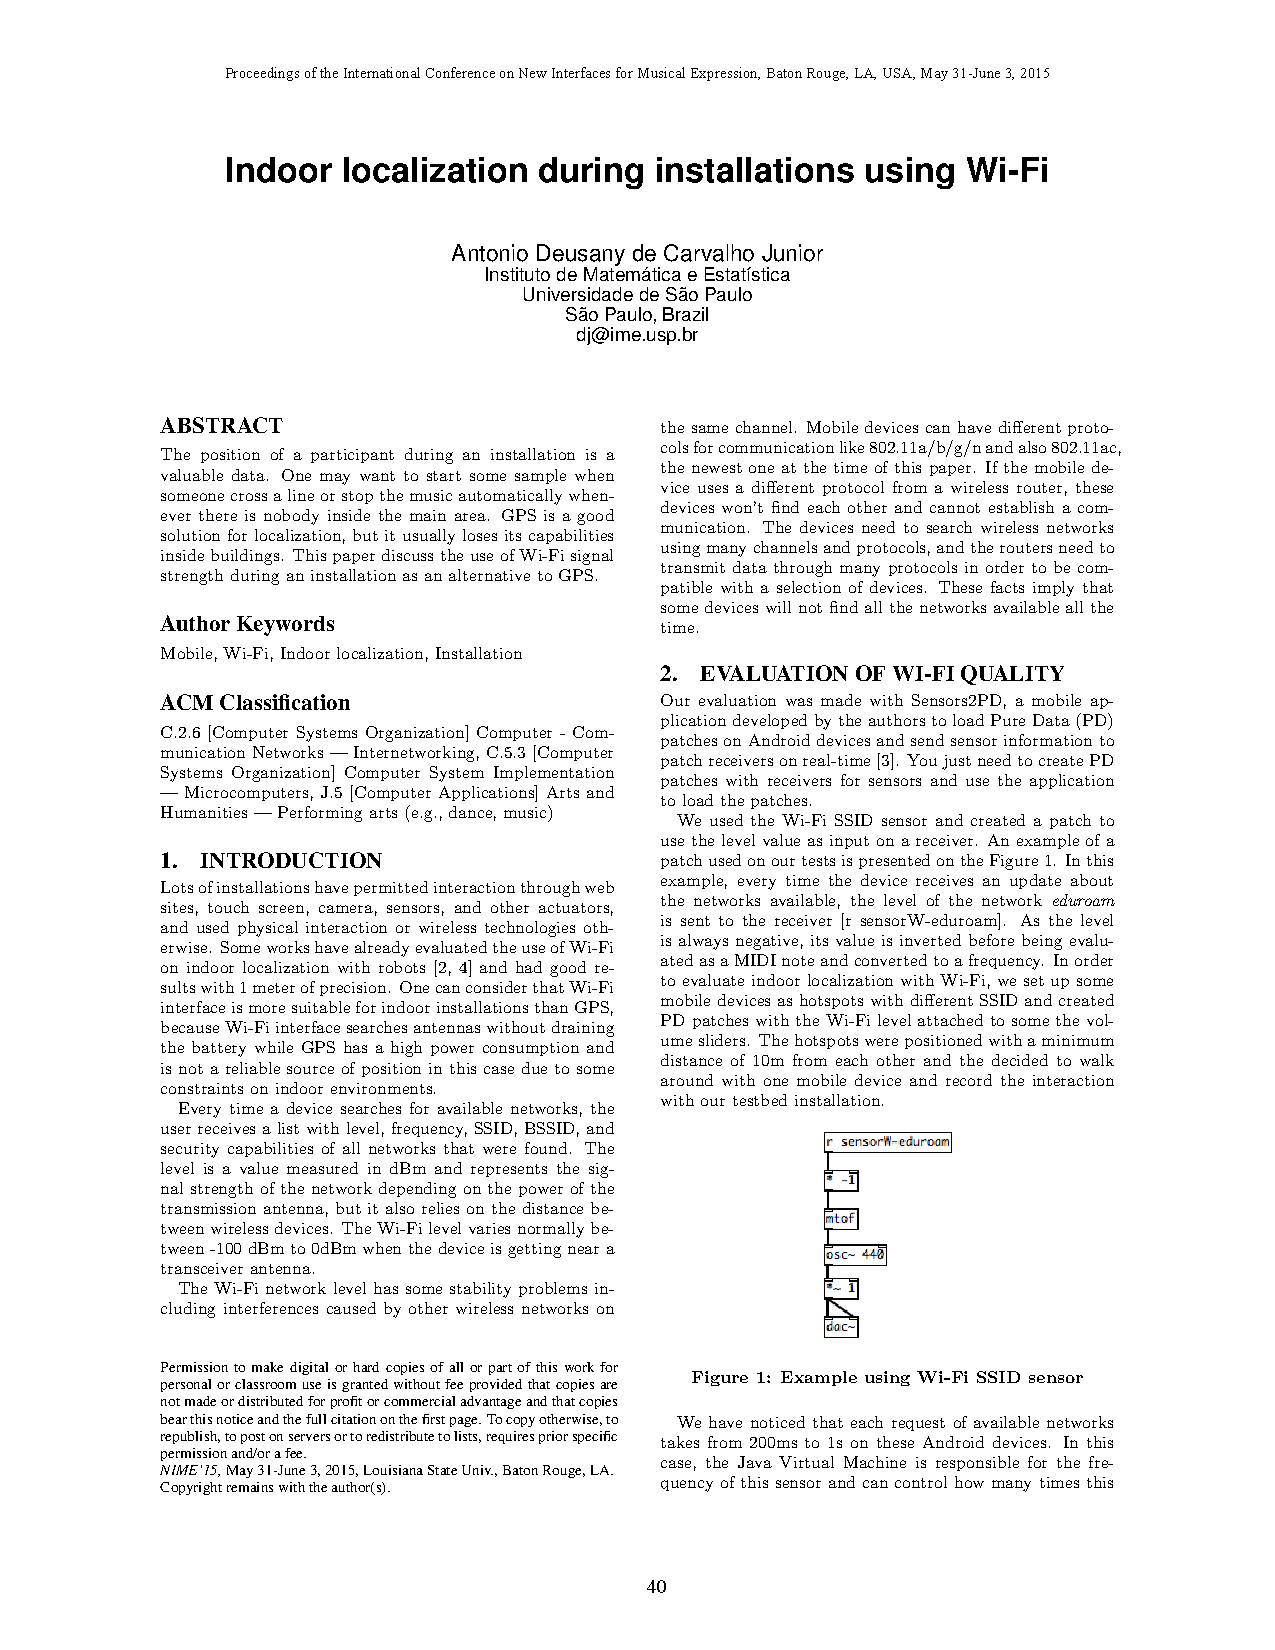
\includepdf[pages=-,frame,scale=0.8,pagecommand={}]{papers/2015-nime.pdf}

%% ------------------------------------------------------------------------- %%
\section{SMC 2015 - Sensors2OSC}
\label{ape:papersmc2015}

\subsection*{Paper details}

Title: \textit{Sensors2OSC}

Authors: Antonio Deusany de Carvalho Junior, Thomas Mayer

\subsection*{Conference details}

Title: 12th Sound and Music Computing Conference

Venue: Maynooth University, Ireland

Dates: July 26 to August 1, 2015

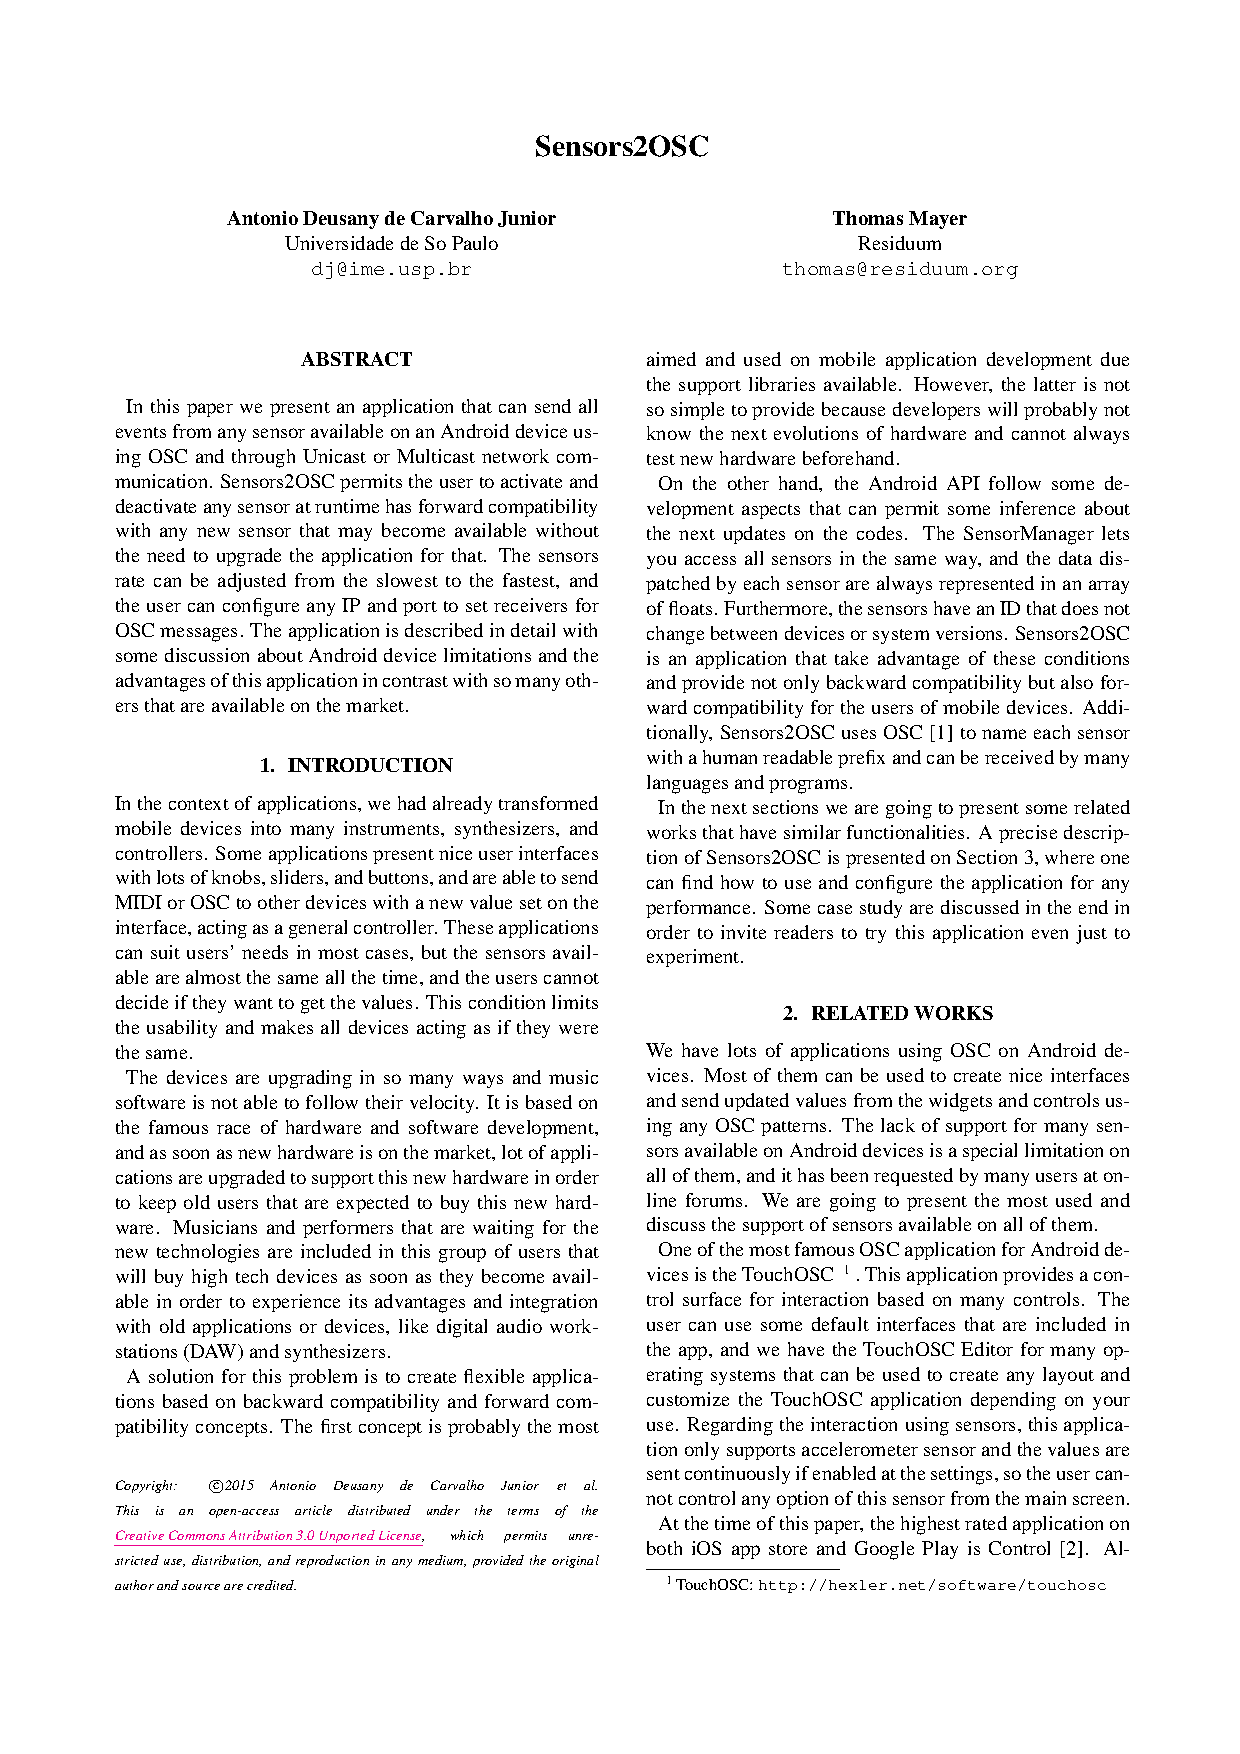
\includepdf[pages=-,frame,scale=0.8,pagecommand={}]{papers/2015-smc.pdf}


%% ------------------------------------------------------------------------- %%
\section{ICMC 2015 - Computer Music through the Cloud: Evaluating a Cloud Service for Collaborative Computer Music Applications}
\label{ape:papericmc2015}

\subsection*{Paper details}

Title: \textit{Computer Music through the Cloud: Evaluating a Cloud Service for Collaborative Computer Music Applications}

Authors: Antonio Deusany de Carvalho Junior, Marcelo Queiroz, Georg Essl

\subsection*{Conference details}

Title: 41st International Computer Music Conference~(ICMC)

Venue: University of North Texas, Denton, TX, USA

Dates: September 25 to October 1, 2015

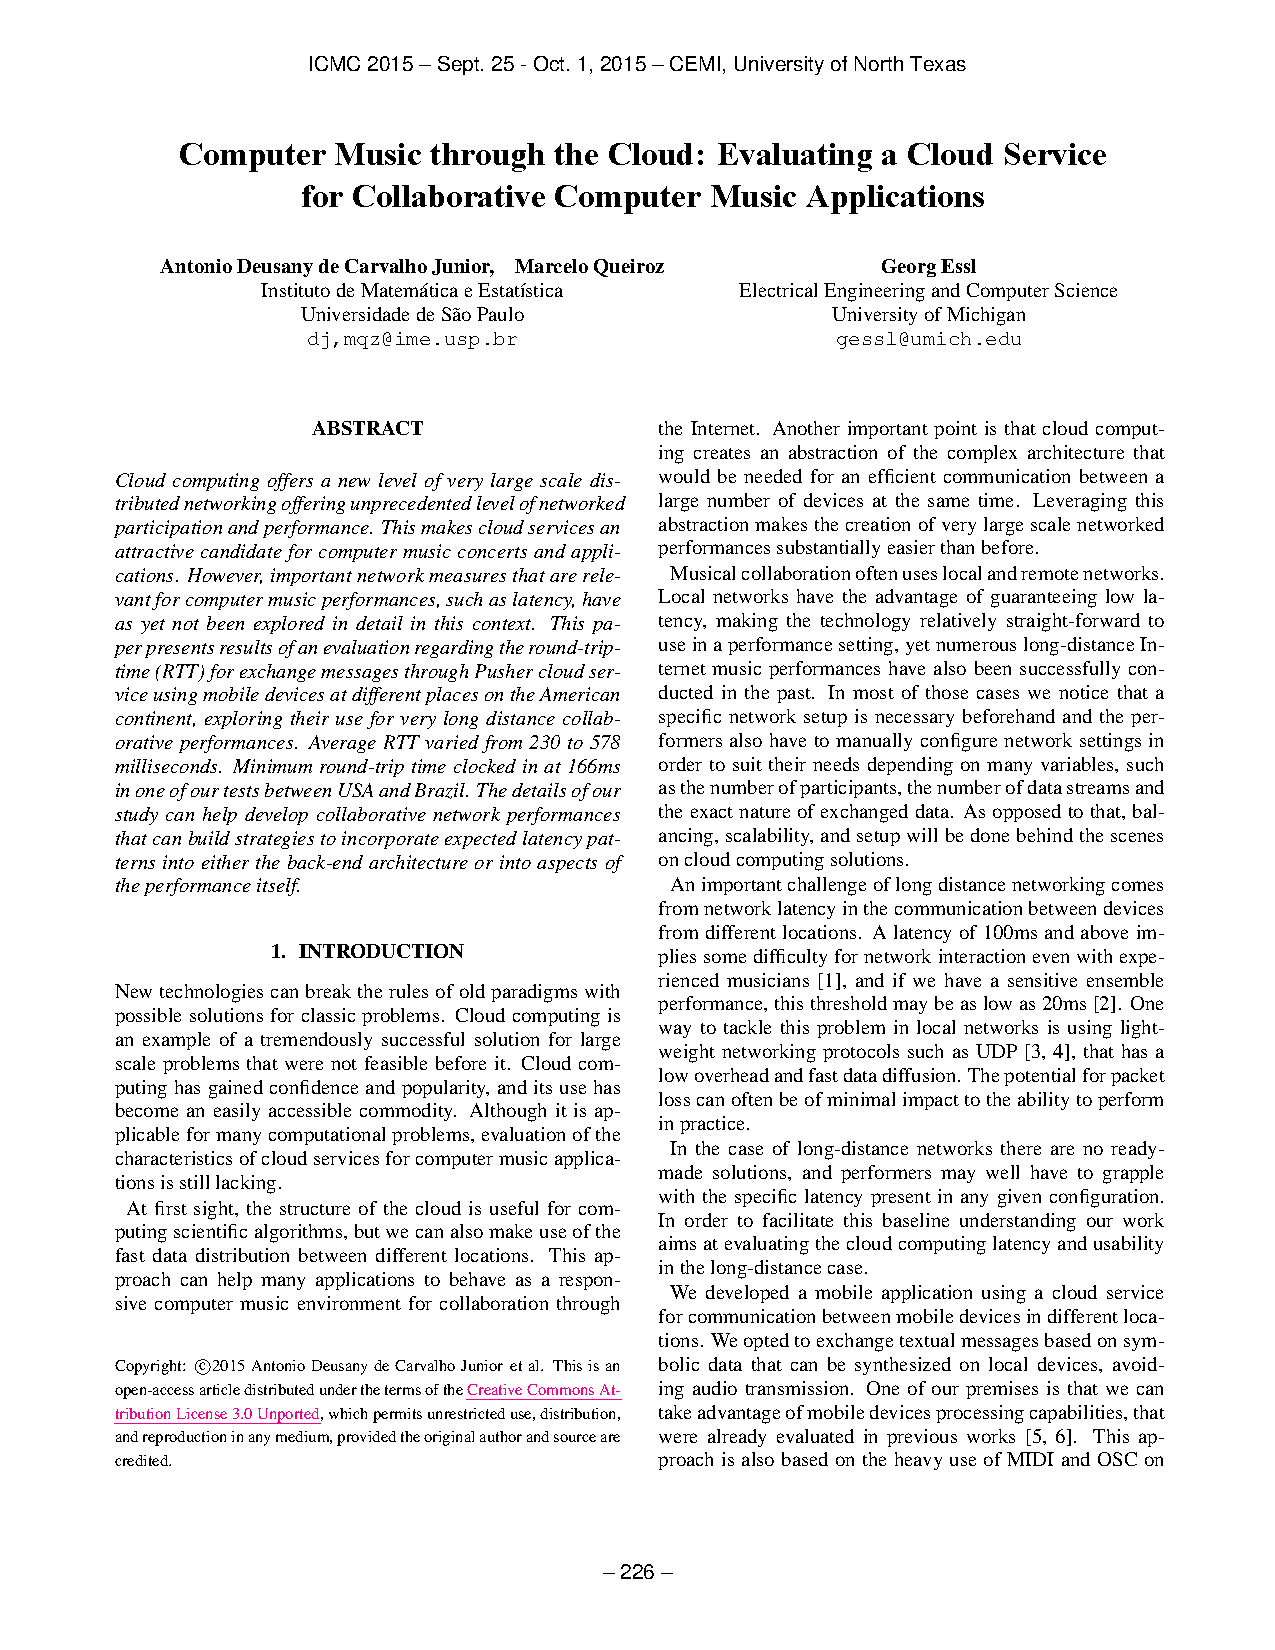
\includepdf[pages=-,frame,scale=0.8,pagecommand={}]{papers/2015-icmc.pdf}

%% ------------------------------------------------------------------------- %%
\section{ICLC 2015 - SuperCopair: Collaborative Live Coding on SuperCollider through the cloud}
\label{ape:papericlc2015}

\subsection*{Paper details}

Title: \textit{SuperCopair: Collaborative Live Coding on SuperCollider through the cloud}

Authors: Antonio Deusany de Carvalho Junior, Sang Won Lee, Georg Essl

\subsection*{Conference details}

Title: International Conference on Live Coding~(ICLC)

Venue: School of Music, University of Leeds, UK

Dates: July 13 to 15, 2015

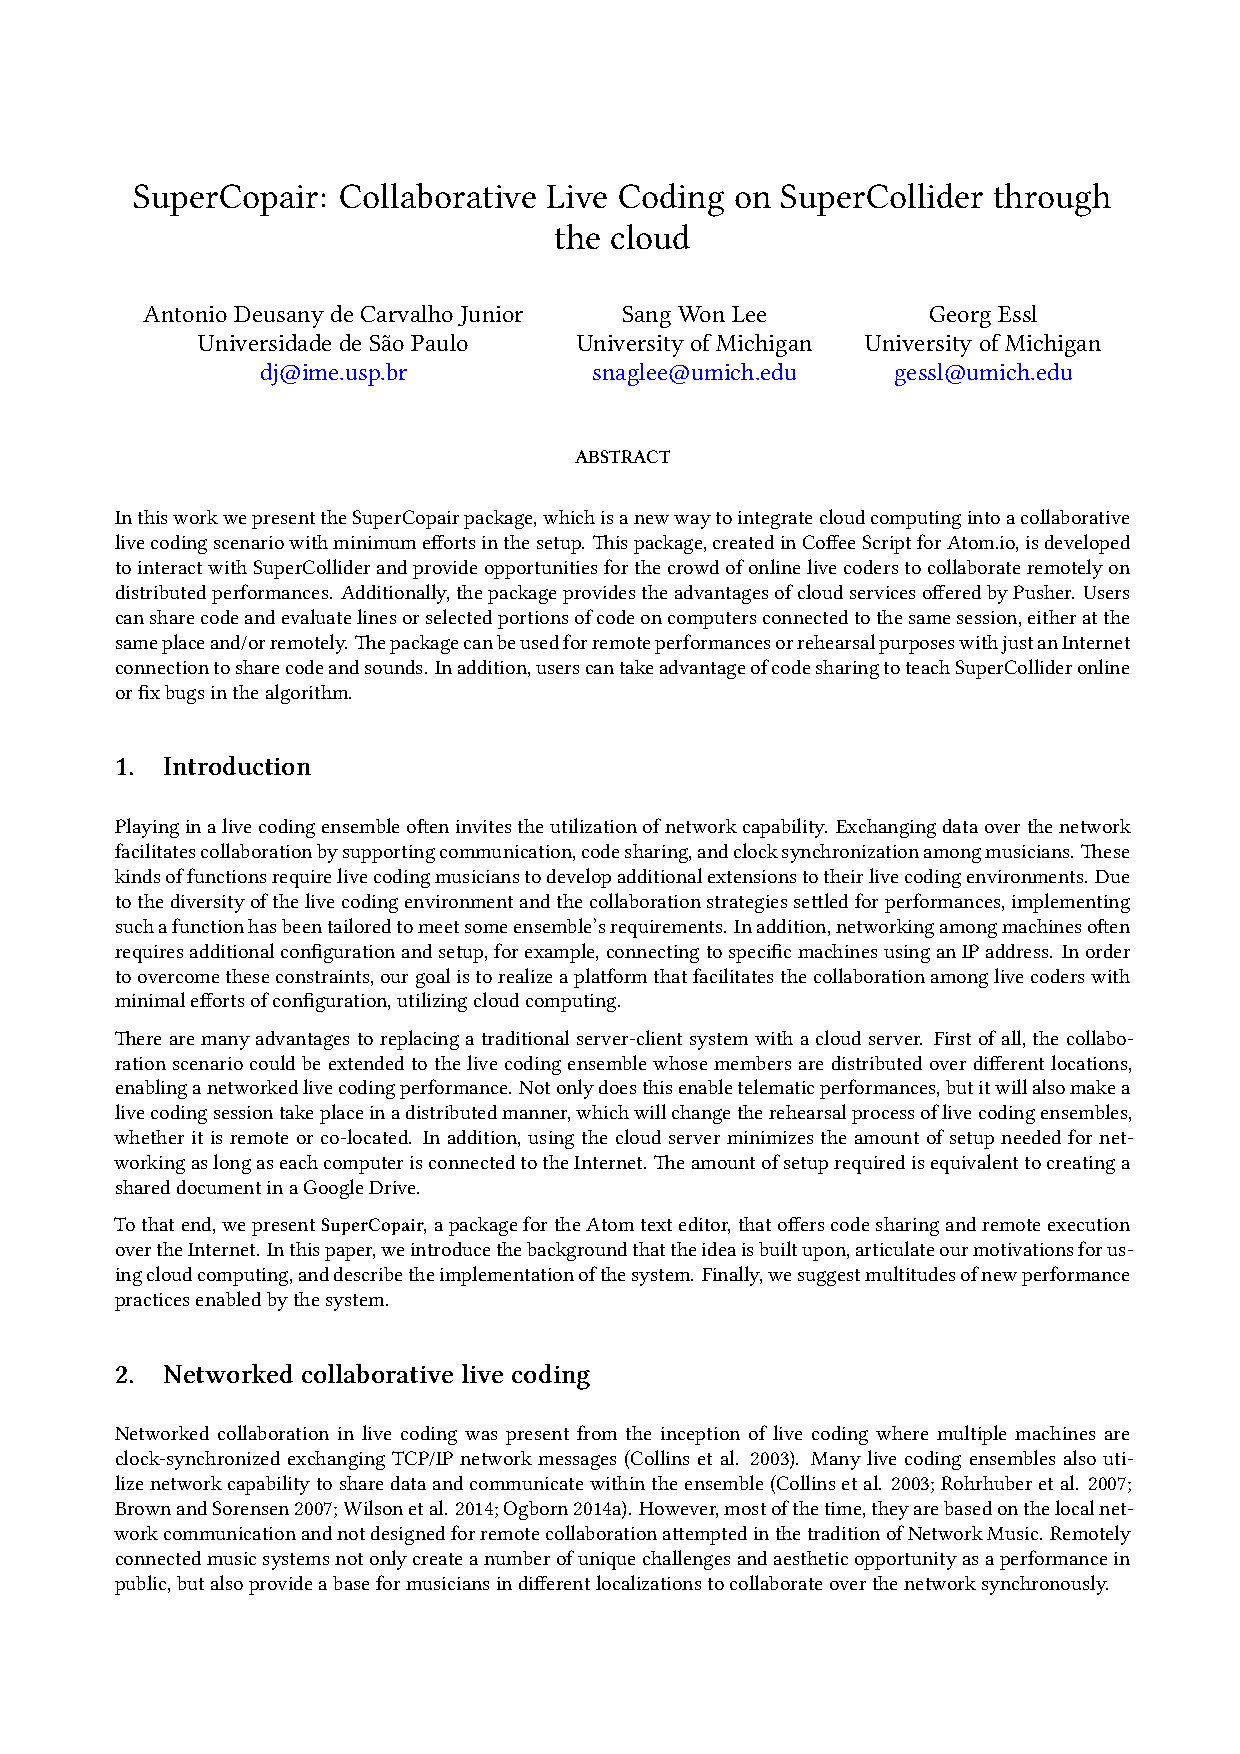
\includepdf[pages=-,frame,scale=0.8,pagecommand={}]{papers/2015-iclc.pdf}

%% ------------------------------------------------------------------------- %%
\section{CLEI 2015 - Cooperative Live Coding as an instructional model}
\label{ape:paperclei2015}

\subsection*{Paper details}

Title: \textit{Cooperative Live Coding as an instructional model}

Authors: Antonio Deusany de Carvalho Junior

\subsection*{Conference details}

Title: XLI Conferencia Latinoamericana en Informática~(CLEI)

Venue: Arequipa, Peru

Dates: October 19 to 23, 2015

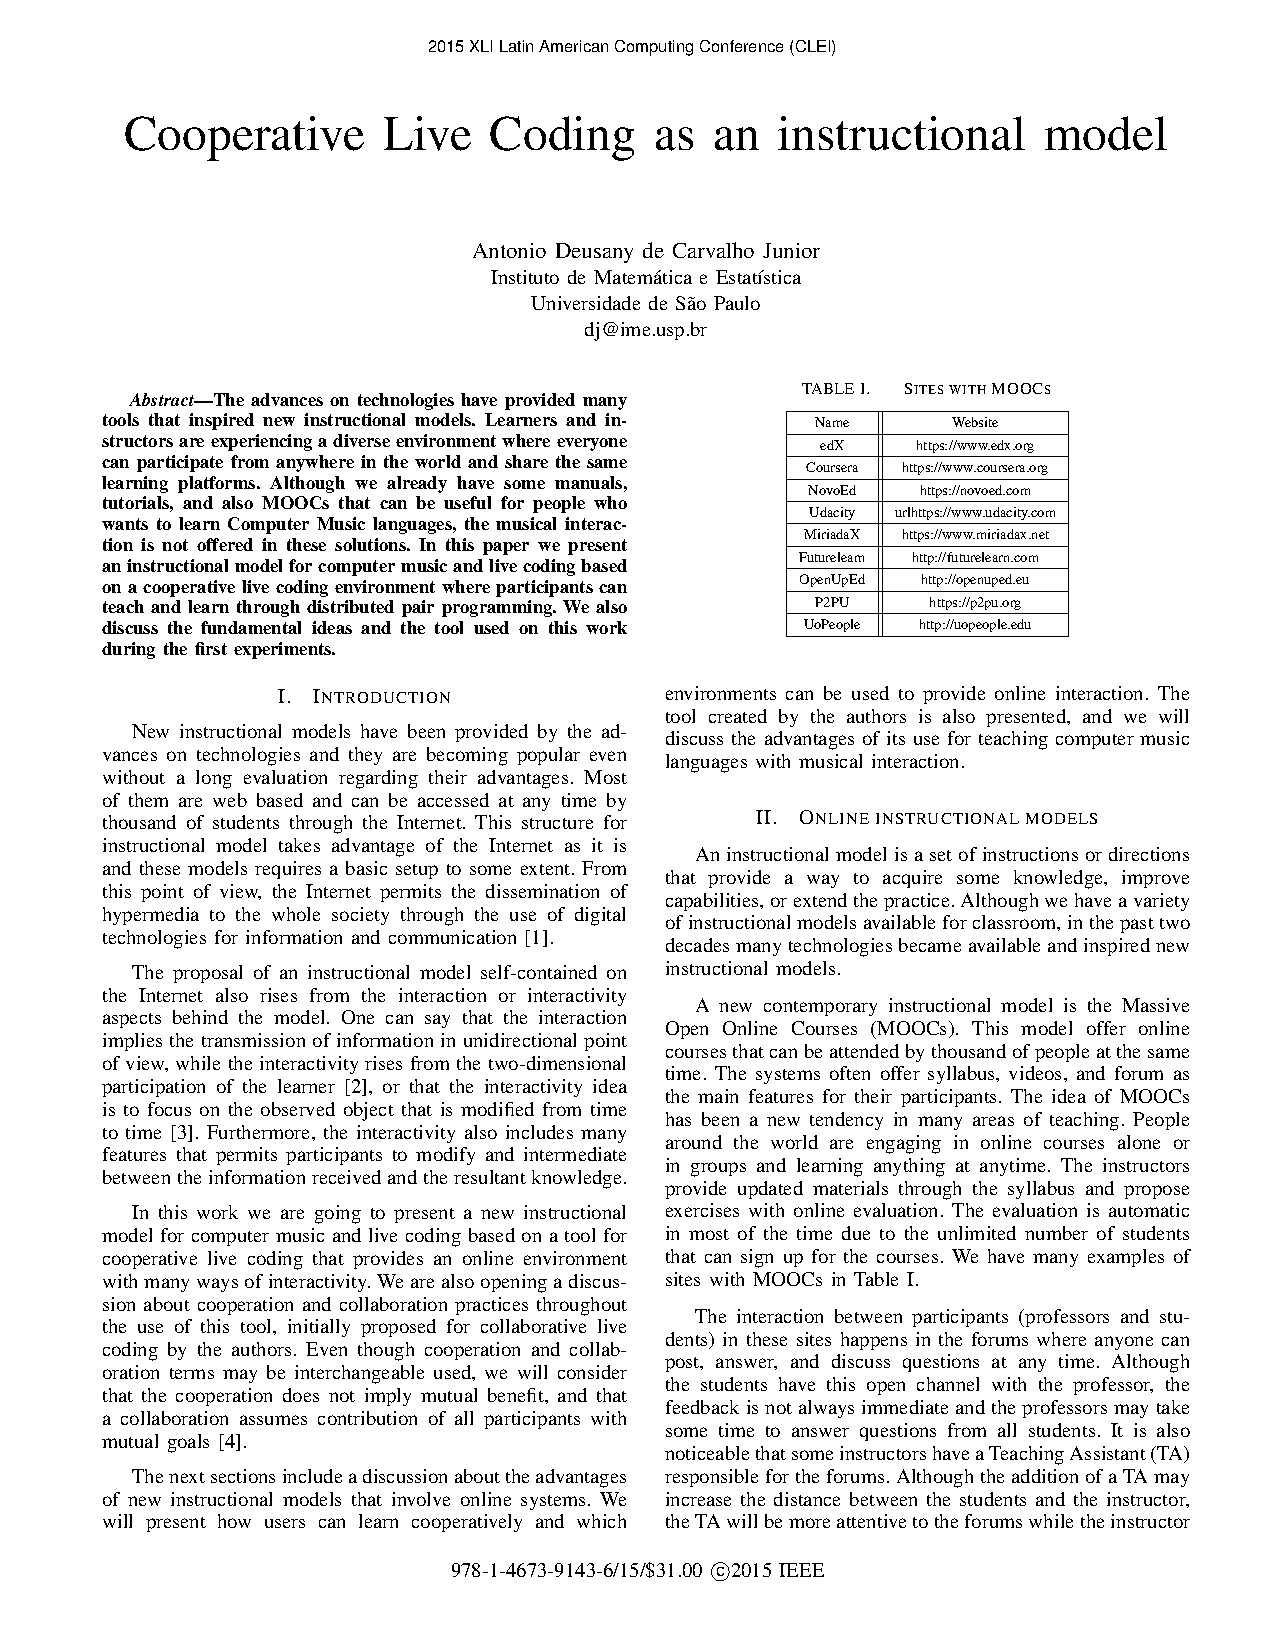
\includepdf[pages=-,frame,scale=0.8,pagecommand={}]{papers/2015-clei.pdf}


%% ------------------------------------------------------------------------- %%
\section{WAC 2016 - Crowd in C[loud]: Audience Participation Music with Online Dating Metaphor using Cloud Service}
\label{ape:paperwac2016}

\subsection*{Paper details}

Title: \textit{Crowd in C[loud]: Audience Participation Music with Online Dating Metaphor using Cloud Service}

Authors: Sang Won Lee, Antonio Deusany de Carvalho Junior, Georg Essl

\subsection*{Conference details}

Title: 2nd Web Audio Conference~(WAC)

Venue: Georgia Tech, Atlanta, GA, USA

Dates: April 4 to 6, 2016

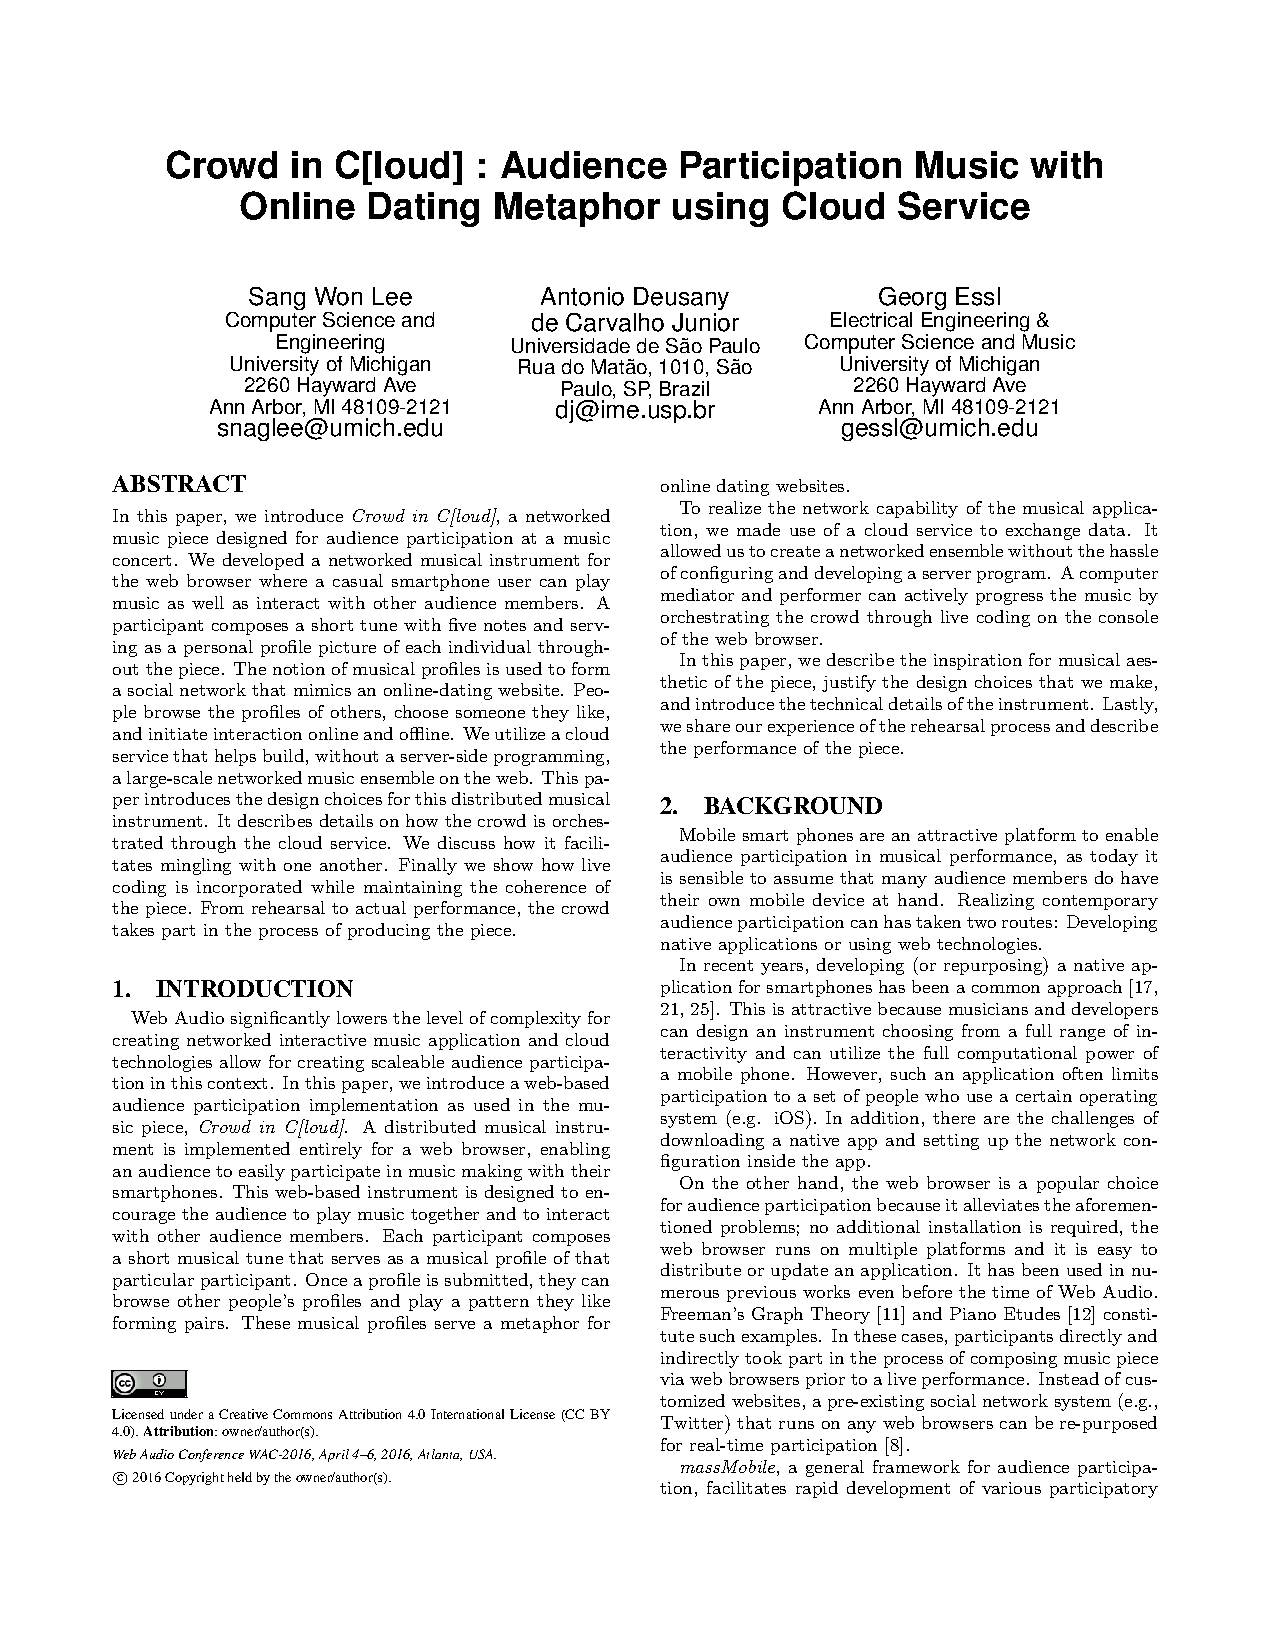
\includepdf[pages=-,frame,scale=0.8,pagecommand={}]{papers/2016-webaudio.pdf}


%% ------------------------------------------------------------------------- %%
\section{NIME 2016 - Understanding Cloud Service in the Audience Music Performance of Crowd in C[loud]}
\label{ape:papernime2016}

\subsection*{Paper details}

Title: \textit{Understanding Cloud Service in the Audience Music Performance of Crowd in C[loud]}

Authors: Antonio Deusany de Carvalho Junior, Sang Won Lee, Georg Essl

\subsection*{Conference details}

Title: 16th International Conference on New Interfaces for Musical Expression

Venue: Griffith University, Brisbane, Australia

Dates: July 11 to 15, 2016

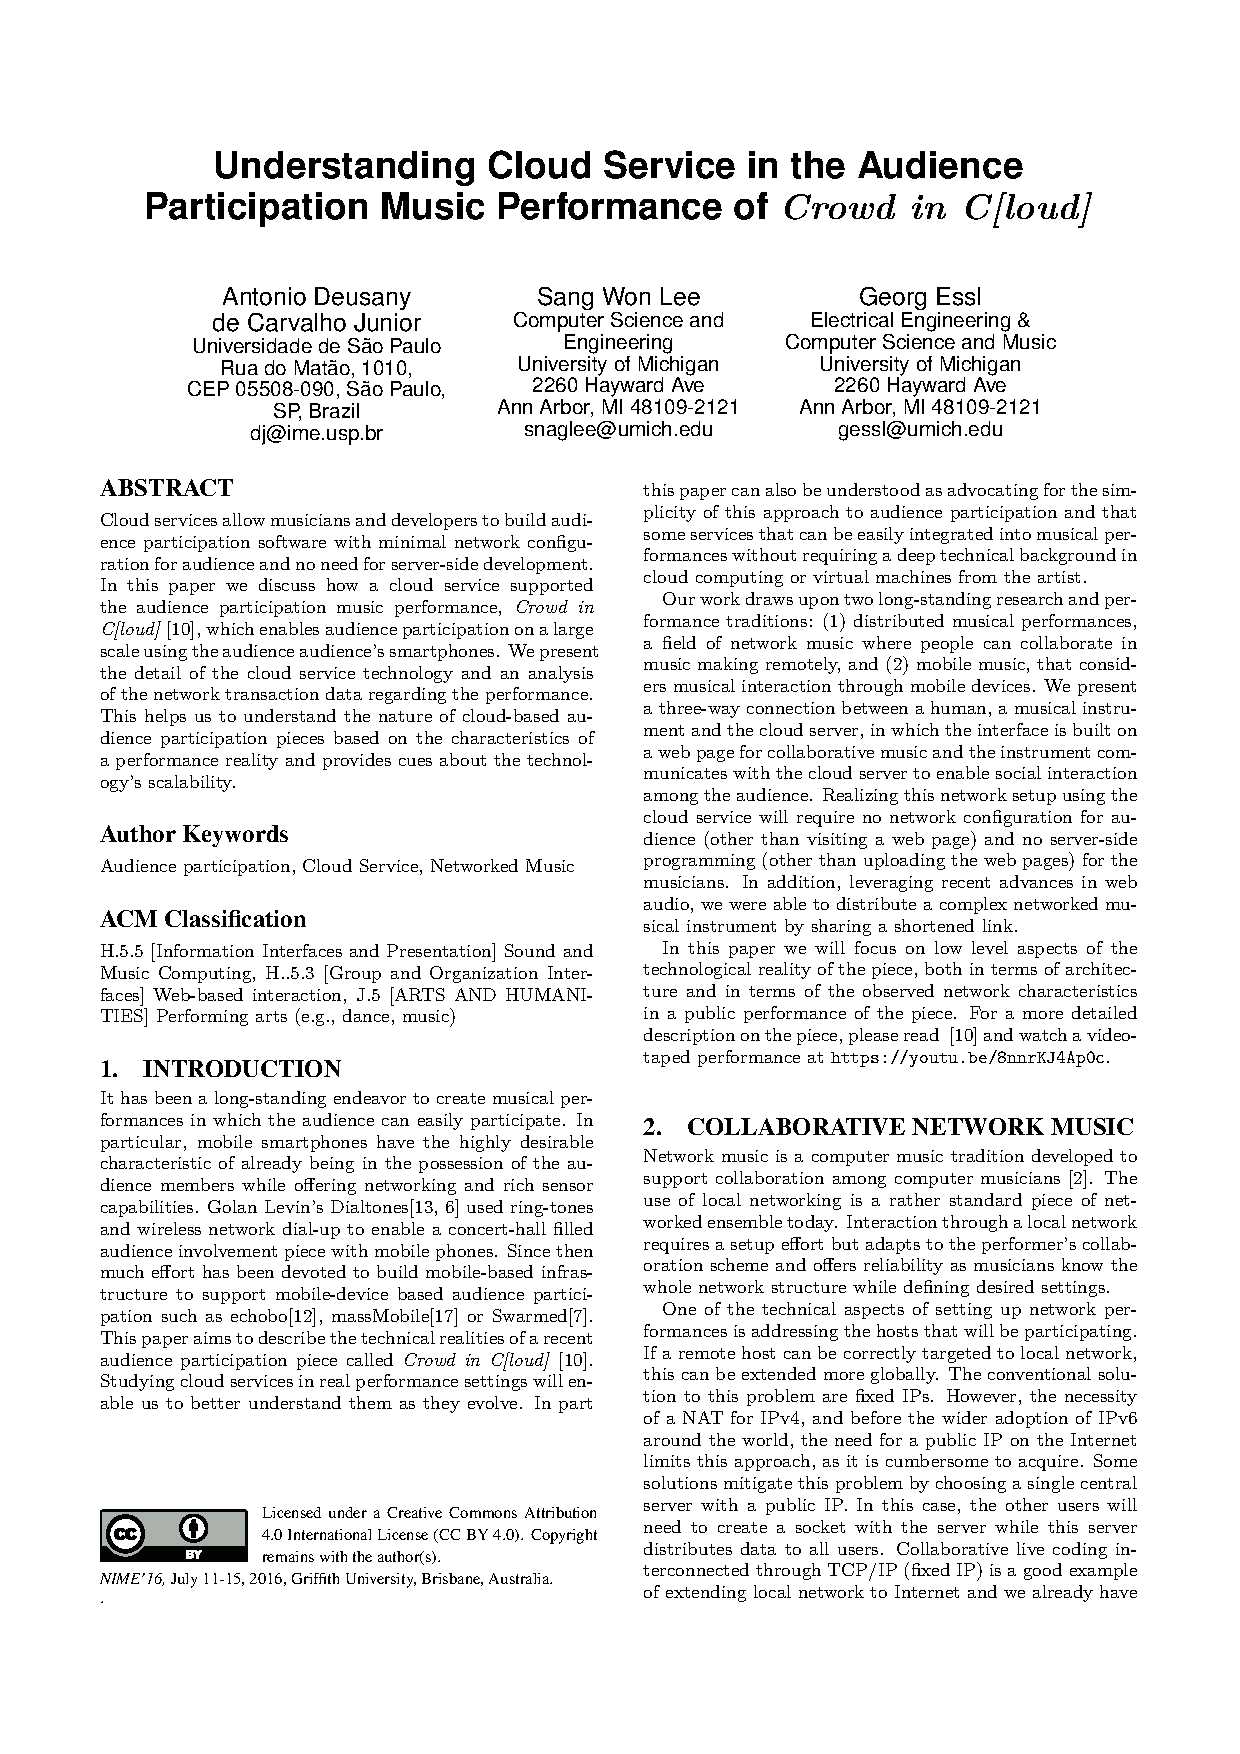
\includepdf[pages=-,frame,scale=0.8,pagecommand={}]{papers/2016-nime.pdf}

%% ------------------------------------------------------------------------- %%
\section{WAC 2017 - Open band: Audience Creative Participation Using Audio Synthesis}
\label{ape:paperwac2017}

\subsection*{Paper details}

Title: \textit{Open band: Audience Creative Participation Using Audio Synthesis}

Authors: Ariane Stolfi, Fábio Goródscy, Antonio Deusany de Carvalho Junior, Fernando Iazzetta, Mathieu Barthet

\subsection*{Conference details}

Title: 3rd Web Audio Conference~(WAC)

Venue: Centre for Digital Music, Queen Mary University of London, London, UK

Dates: August 21 to 23, 2017

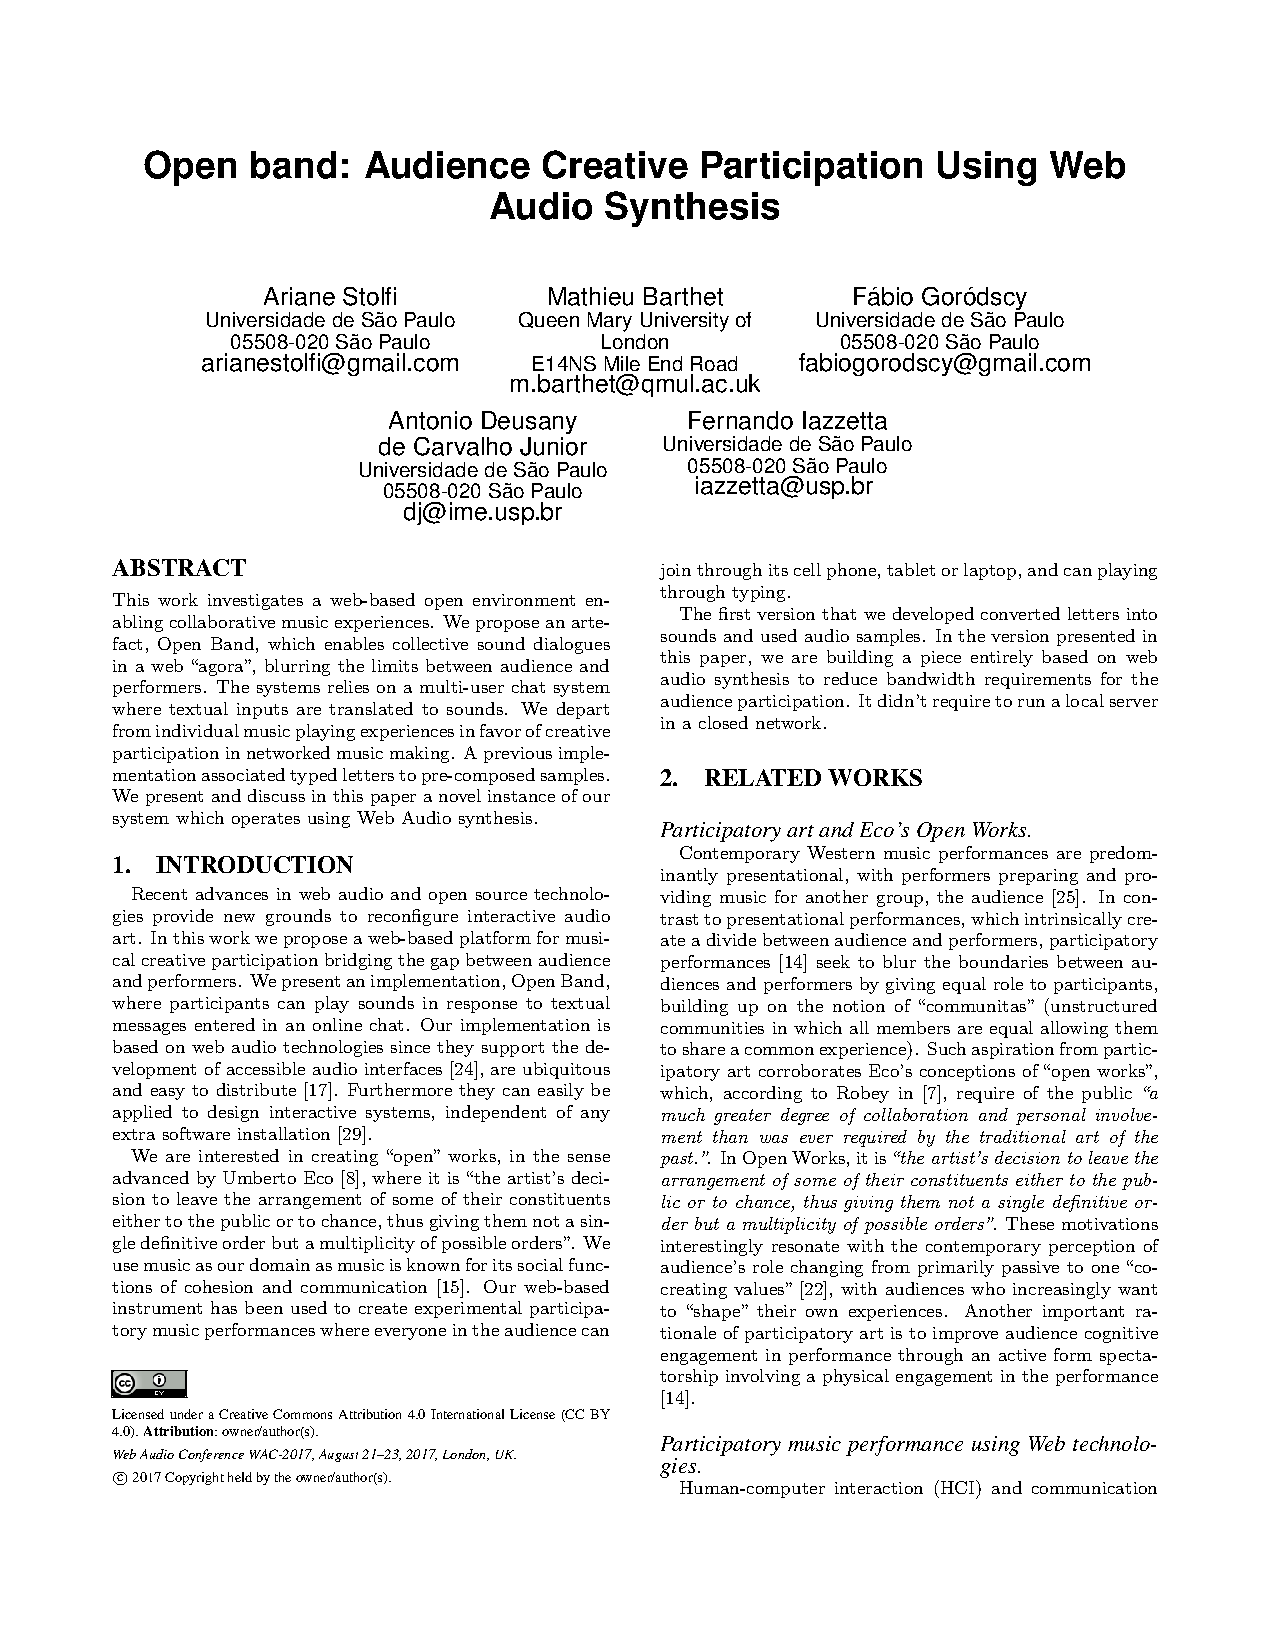
\includepdf[pages=-,frame,scale=0.8,pagecommand={}]{papers/2017-webaudio.pdf}

%% ------------------------------------------------------------------------- %%
\section{Audio Mostly 2017 - Open Band: A Platform for Collective Sound Dialogues}
\label{ape:paperam2017}

\subsection*{Paper details}

Title: \textit{Open band: A Platform for Collective Sound Dialogues}

Authors: Ariane Stolfi, Fábio Goródscy, Antonio Deusany de Carvalho Junior, Mathieu Barthet

\subsection*{Conference details}

Title: Audio Mostly

Venue: Centre for Digital Music, Queen Mary University of London, London, UK
 
Dates: August 23 to 25, 2017

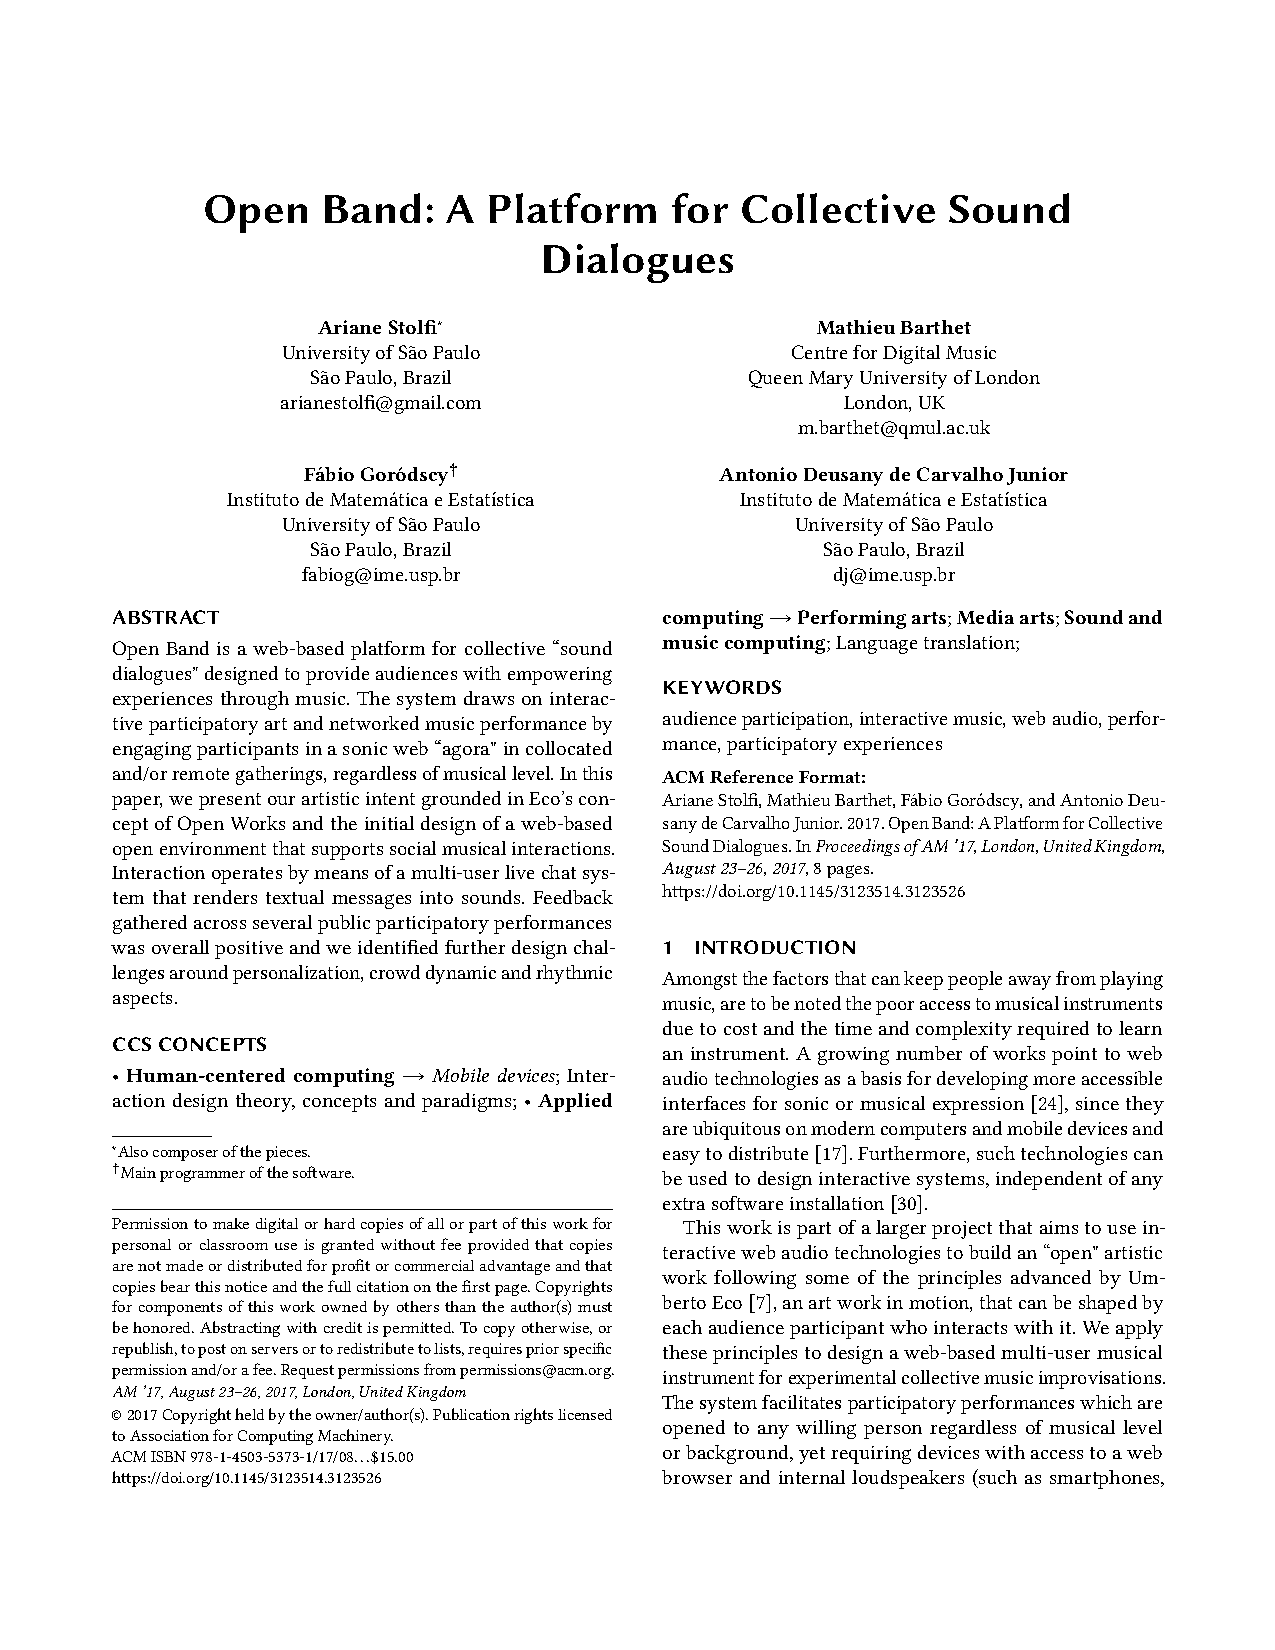
\includepdf[pages=-,frame,scale=0.8,pagecommand={}]{papers/2017-audiomostly.pdf}

	
	% ---------------------------------------------------------------------------- %
	% Bibliografia
	\backmatter \singlespacing   % espaçamento simples
	% \bibliographystyle{alpha-ime} % 
	\bibliographystyle{plainnat-ime} % citação bibliográfica textual
%	 \bibliographystyle{plainnat} % citação bibliográfica textual
	\bibliography{thesisbib}  % associado ao arquivo: 'bibliografia.bib'
	
	% ---------------------------------------------------------------------------- %
	% Índice remissivo
	% \index{TBP|see{periodicidade região codificante}}
	% \index{DSP|see{processamento digital de sinais}}
	% \index{STFT|see{transformada de Fourier de tempo reduzido}}
	% \index{DFT|see{transformada discreta de Fourier}}
	% \index{Fourier!transformada|see{transformada de Fourier}}
	
	% \printindex   % imprime o índice remissivo no documento 
	
\end{document}